\documentclass[11pt]{article}
\usepackage[T1]{fontenc}
\usepackage[margin=1in]{geometry}
\usepackage{amsmath,amssymb,amsthm,mathtools}
\usepackage{booktabs,graphicx,microtype}
\usepackage[round,authoryear]{natbib}
\usepackage[colorlinks=true,allcolors=blue]{hyperref}
\usepackage[nameinlink,noabbrev]{cleveref}
\newtheorem{theorem}{Theorem}[section]
\newtheorem{lemma}[theorem]{Lemma}
\newtheorem{proposition}[theorem]{Proposition}
\newtheorem{corollary}[theorem]{Corollary}
\theoremstyle{definition}
\newtheorem{definition}[theorem]{Definition}
\newtheorem{example}[theorem]{Example}
\theoremstyle{remark}
\newtheorem{remark}[theorem]{Remark}
% All derivatives and matrix inequalities use the fixed tangent-space metric.
\newcommand{\R}{\mathbb R}
\newcommand{\V}{\mathcal V}
\newcommand{\BV}{\mathbb B_{\mathcal V}}
\newcommand{\OPT}{\operatorname{OPT}}
\newcommand{\ri}{\operatorname{ri}}
\newcommand{\aff}{\operatorname{aff}}
\newcommand{\diam}{\operatorname{diam}}
\newcommand{\tr}{\operatorname{tr}}
\newcommand{\Diag}{\operatorname{Diag}}
\newcommand{\norm}[1]{\left\lVert #1\right\rVert}
\newcommand{\inner}[2]{\left\langle #1,#2\right\rangle}
\DeclareMathOperator*{\argmin}{arg\,min}

\title{Objective Sublevels and Central-Path Hessian Conditioning}
\author{}
\date{}
\begin{document}
\maketitle
\begin{abstract}
We characterize the equality-reduced primal barrier Hessian by the
geometry of objective sublevels in a fixed Euclidean metric. For a
compact convex feasible set, a nonconstant linear objective, and any
finite-parameter self-concordant barrier, the unit Dikin ellipsoid at
a central point of primal gap $g$ is comparable with the difference
body $L(g)-L(g)$. This yields a Loewner comparison between different
barriers at equal gap and the matching law
$\kappa(g)=\Theta((\operatorname{diam}L(g)/g)^2)$.
Explicit constants extend the results to points with Newton decrement
below one and to uniformly bounded families of barrier parameters.
Directional widths determine every ordered spectral scale. We derive
conditioning regimes, a uniform near-degeneracy plateau, and four exact
leading eigenvalue constants for the reduced log-Hessian of a classical
$3\times3$ semidefinite construction. A paired section shows that
singularity degree does not determine the conditioning exponent.
For linear programs, every fixed barrier has at most two spectral scales;
its weak eigenspace approaches the optimal-face tangent at rate $O(g)$,
improved to $O(g^2)$ for the logarithmic barrier. A globally certified
example attains the general rate and separates small discarded residual
from accurate Newton direction recovery. We state the resulting
clustered-CG consequence and the additional assumptions needed for
quantum solver interpretations. Reproducible computations include exact
rational input certificates and explicit precision screens.
\end{abstract}
\noindent\textbf{Keywords:} self-concordant barriers; central path;
Hessian conditioning; objective sublevels; semidefinite programming;
spectral clustering.
\section{Introduction}
\label{sec:introduction}

The Newton systems of interior-point methods are built from the
Hessian of a self-concordant barrier, directly or through a Schur
complement or an augmented system, and can become increasingly
ill-conditioned as the requested objective accuracy improves. This is
usually analyzed for the
logarithmic barrier or for a particular primal--dual linear system. We
ask how much of it is already forced by the feasible set and the
objective. Can a different barrier, with a different central path,
improve the growth rate of the condition number of the primal barrier
Hessian? Which geometric features determine the
individual eigenvalues? The answers matter when choosing a barrier and
when interpreting solver costs that depend on the condition number.

We answer these questions for the primal barrier Hessian restricted to
the tangent space of the affine constraints (the reduced Hessian), in a
fixed Euclidean metric. Let $P$ be a compact convex feasible set with
nonempty relative interior, and let the linear objective
$\inner{c}{x}$, to be minimized, be nonconstant on the affine hull of
$P$. Let $L(g)$ be the set of feasible points whose objective value
exceeds the optimal value by at most $g$ (the primal objective gap), and let $D(g)=\diam L(g)$. For a barrier $F$, let
$\widehat H_F(g)$ be the Hessian of $F$ (not of $\mu F$) at the central
point with gap $g$, that is, at the minimizer of
$F(x)+\inner{c}{x}/\mu$ whose gap is $g$. With $\kappa$ the ratio of the largest to the smallest eigenvalue,
our main conclusion is
\begin{equation}
 \kappa\bigl(\widehat H_F(g)\bigr)
 =\Theta\!\left(\frac{D(g)^2}{g^2}\right)
 \qquad(g\downarrow0)
 \label{eq:intro-diameter-law}
\end{equation}
for every fixed self-concordant barrier $F$ with finite barrier
parameter. The constants may depend on the fixed instance, the metric,
and the barrier parameter, but not on $g$. Changing the barrier can
change the constants and the central points, but not the rate, which is
determined by the geometry of the objective sublevel sets.

The diameter law \eqref{eq:intro-diameter-law} follows from a stronger
comparison. Let $E_F$ be the unit Dikin ellipsoid of $F$ at a point,
taken in the tangent space, and let $K_g=L(g)-L(g)$ be the difference
body of the sublevel set, which depends on neither the barrier nor the
point. Suppose that, at a point
with gap $g$, the Newton decrement $\rho$ of $F+\inner{c}{x}/\mu$,
measured in the Hessian of $F$, is less than one for some $\mu>0$. Then
$E_F\subset K_g\subset2CE_F$ at this point, where $\nu$ is the barrier
parameter and
\[
 C=\frac{\nu+2\sqrt\nu+\rho}{1-\rho},\qquad 0\leq\rho<1.
\]
Since $K_g$ has diameter $2D(g)$, and the largest ball centered at the
origin inside $K_g$ has radius of order $g$, this containment gives
\eqref{eq:intro-diameter-law}.

\subsection{Main results}

\begin{enumerate}
\item \textit{Comparison at equal objective accuracy.}
\Cref{thm:difference-body,thm:diameter-law,thm:radial-spectrum} prove
the containment, the resulting Loewner-order comparison of the
Hessians of different barriers at equal gap, the diameter law, and
bounds on every eigenvalue: the $j$th eigenvalue lies between the inverse squares
of two minimax radial widths of $K_g$, up to the factor $4C^2$. The estimates
hold uniformly over barriers with bounded parameters and Newton
decrements bounded uniformly below one (\cref{cor:uniform-rates}).
On an unbounded feasible set, the pointwise bounds hold at the points of
any compact objective sublevel set (\cref{prop:localization}).
The finite barrier parameter is needed: \cref{sec:formulation-scope}
gives a self-concordant function without one for which the law fails.
\item \textit{Sharp geometric and spectral examples.}
The law gives bounded conditioning at every unique optimum of a
polytope, including degenerate vertices, and conditioning of order
$g^{-2}$ when the optimal face has positive dimension
(\cref{prop:three-regimes}). For a fixed simplex and objectives
$c_\vartheta$ whose optimum is a unique vertex for $\vartheta>0$ and an
edge at $\vartheta=0$, the condition number is
$\Theta(\min\{\vartheta^{-2},g^{-2}\})$ uniformly in $\vartheta$
(\cref{prop:simplex-plateau}). For a
trace-normalized version of a classical $3\times3$ semidefinite program,
\cref{thm:fractional-spectrum} gives the asymptotics of all four
eigenvalues of the reduced log-barrier Hessian, with exact constants.
Adding two linear constraints gives a problem whose optimality system
has the same singularity degree, two, but on which every fixed barrier
has condition number $\Theta(g^{-1})$ instead of $\Theta(g^{-3/2})$
(\cref{prop:paired-sdp}). Thus singularity degree alone does not
determine the conditioning exponent.
\item \textit{Newton right-hand sides, and what condition numbers do
not show.} For a linear program with an optimal face of dimension $f$,
every fixed barrier Hessian at the central point with gap $g$ has $f$
eigenvalues of order one and the others of order $g^{-2}$. The
orthogonal projector onto the eigenspace of the $f$ small eigenvalues (the weak eigenspace)
differs in norm from the projector onto the tangent space of the optimal
face by $O(g)$, and by $O(g^2)$ for the logarithmic barrier
(\cref{thm:lp-all-spectra}). Hence, at an exact central point, the
Newton right-hand side has a component of relative norm $O(g)$ in that
eigenspace, and $O(g^2)$ for the logarithmic barrier. An explicit $20$-self-concordant barrier
on a rectangle attains the rate $O(g)$ along a sequence of gaps
(\cref{prop:oscillatory-barrier}). For this barrier, discarding that
right-hand-side component, although its relative size tends to zero,
produces a solution whose relative Euclidean error tends to one.
For spectra in two clusters, \cref{prop:clustered-cg} bounds the
number of conjugate-gradient iterations in exact arithmetic.
\end{enumerate}

\subsection{Relation to prior work}

The geometry of self-concordant barriers is classical
\citep{nesterov1994,renegar2001,nesterov2018}; we give short proofs of
the facts we use (Dikin containment, semiboundedness, and asymmetric
containment) to fix our constants.
\citet[Proposition 2.3.2(iii), equation (2.3.9)]{nesterov1994} compares
the local Hessian norm with the symmetric chord radius at a fixed
interior point, and so already compares the Hessians of different
barriers at the \emph{same point}. We compare Hessians at generally
different points, by comparing each with the same difference body $K_g$,
which does not depend on the point.
\citet{freund2003} studies the geometry of primal--dual level sets.
More directly, \citet[Section 5.1, Fact 5.2 and Remark
5.1]{xiongfreund2024} use central-path ellipsoids to relate the diameter
and conic radius of primal--dual sublevel sets to Hessian eigenvalues,
in order to analyze rescaling for PDHG; their work is a direct
antecedent of our geometric method. We instead compare the primal
Hessian on the tangent space with the difference body $K_g$ at a
prescribed primal gap, and obtain the diameter law and the comparison
between barriers.

\citet{renegar1996} relates the conditioning of the linear equations of
barrier methods to problem conditioning and to conjugate-gradient
solution, and \citet{pena2001,pena2002} develops a primal--dual
condition-number approach and implicit-barrier methods.
\citet[Proposition 3.2]{pena2002} parameterizes the central
path by the primal objective gap, and his Section 3.3 bounds the
condition number of the Schur matrix $A\nabla^2F(x)^{-1}A^\top$ by an
inverse-square rate in the gap, under his assumptions. We therefore
claim novelty neither for the gap parameterization nor for an
inverse-square upper bound as such; for the reduced Hessian, we
add the two-sided dependence on $D(g)$ and the comparison
between barriers.

Spectral splitting of logarithmic-barrier Hessians and its numerical
consequences were studied by \citet{wright1994,wright1998};
\citet{forsgren2002} surveys interior methods, and
\citet{wrightorban2002} treat degenerate nonlinear programs. Limits of
LP central paths and their analytic properties are classical
\citep{adler1991,guler1994,halicka1999}; our limit of the log-barrier
Hessian scaled by $\mu^2$ at a unique LP optimum, including a
degenerate vertex, is a corollary of this theory.
\citet{duistermaat2001} analyzes the boundary asymptotics of the Hessian
Riemannian structure under additional smoothness assumptions; his Remark
2.3 gives oscillatory self-concordant perturbations, and qualitative
nonconvergence of central paths has earlier examples
\citep{boltepauwels2022}. Our LP contributions are the eigenvalue orders
for arbitrary finite-parameter barriers, the rates for the
small-eigenvalue eigenspace, and, for the oscillatory example, the
sharpness of the rate $O(g)$ and the calculation of the solution error.

For semidefinite programming, error bounds and facial reduction connect
singularity degree with fractional powers
\citep{sturm2000,drusvyatskiy2017,lourenco2021}. We use a
trace-normalized version of Sturm's classical $3\times3$ example and do
not claim a new source of error bounds with exponent $1/4$.
\citet{alizadeh1998} study a primal--dual Schur matrix, \citet{wei2010}
investigate instances where strict complementarity fails, and
\citet{sremac2021} relate singularity degree to primal and dual spectral
rates along a regularization path whose constraints change with the
path parameter. Our equality constraints, and hence the tangent space of
our Hessian, are fixed; \cref{sec:fractional-sdp} compares the paths and
matrices in detail.

Finally, condition numbers alone do not determine solver cost.
Cluster-sensitive conjugate-gradient analysis is classical
\citep{axelsson1994}; we give an explicit polynomial bound on the
energy-norm error in exact arithmetic, in the form needed here. Quantum
linear-system results also depend on access to the matrix,
normalization, preparation of the right-hand side, and the required
output \citep{gilyen2019,orsucci2021}, including in quantum
interior-point methods such as the quantum speedups for LP of
\citet{apersgribling2026}. We do not derive an end-to-end quantum lower
bound from the diameter law.

To the best of our knowledge, the equal-gap comparison between
arbitrary finite-parameter barriers, with bounds that depend explicitly
on the Newton decrement, and the resulting two-sided characterization by
the diameter have not previously been stated in this form. Our other
contributions are the explicit calculations listed above and their
consequences for all barriers.

\subsection{Organization}

\Cref{sec:setup,sec:geometry,sec:widths} develop the general theory,
\cref{sec:classifications,sec:lp-limits,sec:fractional-sdp} give
classifications and exact examples,
\cref{sec:lp-spectra,sec:clustered-solves} treat Newton right-hand
sides and linear solves, and \cref{sec:formulation-scope} explains the
roles of the metric, the formulation, and the finite barrier parameter.
\Cref{sec:numerics} gives reproducible numerical illustrations with
exact rational certificates of their input hypotheses; the claims they
illustrate are proved earlier.

\section{The objective gap and the reduced Hessian}
\label{sec:setup}

In the main geometric results, $P$ is a compact convex subset of a
finite-dimensional Euclidean space, with affine hull $x^0+\V$ and relative
interior $P^\circ=\ri P$. The tangent space $\V$ has dimension $d\geq1$.
We minimize a linear functional $\inner{c}{x}$ that is nonconstant on $P$;
equivalently, its orthogonal projection $c_{\V}$ onto $\V$ is nonzero. Set
\begin{align}
 \OPT&=\min_{x\in P}\inner{c}{x}, &
 \Phi&=\{x\in P:\inner{c}{x}=\OPT\},\label{eq:optimum}\\
 g(x)&=\inner{c}{x}-\OPT, &
 \Delta&=\max_{x\in P}g(x)>0.\label{eq:gap-range}
\end{align}
For $0\leq g\leq\Delta$, define
\begin{equation}
 L(g)=\{y\in P:g(y)\leq g\},\qquad
 D(g)=\diam L(g),\qquad K_g=L(g)-L(g)\subset\V.
 \label{eq:sublevels}
\end{equation}
The difference body $K_g$ consists of all chords of the sublevel set,
translated to the origin. Unlike the diameter, it records the longest
chord in every direction. For an interior point $x$, also put
\begin{equation}
 \ell(x)=\max_{y\in L(g(x))}\norm{y-x},\qquad
 \frac{D(g(x))}{2}\leq\ell(x)\leq D(g(x)).
 \label{eq:chord-length}
\end{equation}
The lower inequality follows from the triangle inequality applied to a
pair of points at distance $D(g(x))$.

\begin{definition}[Barrier and metric]
\label{def:barrier}
A $\nu$-self-concordant barrier for $P$, with $\nu>0$, is a convex
$C^3$ function $F:P^\circ\to\R$ that tends to $+\infty$ at every relative
boundary point, has positive-definite tangent Hessian, and satisfies
\begin{align}
 |D^3F(x)[h,h,h]|&\leq2\bigl(D^2F(x)[h,h]\bigr)^{3/2},\label{eq:sc}\\
 |DF(x)[h]|&\leq\sqrt\nu\bigl(D^2F(x)[h,h]\bigr)^{1/2}
 \qquad(h\in\V).\label{eq:barrier-gradient}
\end{align}
All gradients and Hessians below are taken along the affine space
$x^0+\V$, that is, in directions $h\in\V$. Write $H_F(x)$ for the
self-adjoint operator on $\V$ representing $D^2F(x)$; we call it the
reduced Hessian. Define
\begin{equation}
 \norm{h}_x=\sqrt{\inner{H_F(x)h}{h}},\qquad
 \norm{v}_x^*=\sqrt{\inner{H_F(x)^{-1}v}{v}},\qquad
 E_F(x)=\{h\in\V:\norm{h}_x\leq1\}.
 \label{eq:local-metric}
\end{equation}
The condition number is
$\kappa_F(x)=\lambda_{\max}(H_F(x))/\lambda_{\min}(H_F(x))$.
\end{definition}

If $W$ is an orthonormal basis matrix for $\V$, the matrix of this operator
is $W^\top\nabla^2F(x)W$; its eigenvalues do not depend on the choice of
orthonormal basis. The Euclidean metric is fixed throughout. For symmetric
matrix variables it is the Frobenius metric, and for several blocks it is
the product Frobenius metric. We use the Hessian of $F$, not of $\mu F$.
Multiplying by $\mu$ leaves the condition number unchanged but multiplies
every eigenvalue by $\mu$. A different representation of the feasible set,
or a nonorthogonal change of coordinates, needs a separate analysis of
the metric.

\subsection{Two standard barrier facts, with proofs}

The following facts are standard properties of self-concordant barriers
\citep{nesterov1994,renegar2001}. We give short one-dimensional proofs
to fix the normalization and the treatment of boundary points.

\begin{lemma}[Dikin containment and semiboundedness]
\label{lem:standard-containment}
For $x\in P^\circ$,
\begin{equation}
 x+\operatorname{int}_{\V} E_F(x)\subset P^\circ,
 \qquad x+E_F(x)\subset P,
 \label{eq:dikin}
\end{equation}
and for every $y\in P$,
\begin{equation}
 \inner{\nabla F(x)}{y-x}\leq\nu.
 \label{eq:semiboundedness}
\end{equation}
In particular, at every interior point, whether central or not,
\begin{equation}
 \norm{c_{\V}}_x^*\leq g(x).
 \label{eq:objective-support}
\end{equation}
\end{lemma}

\begin{proof}
Fix $h\in\V$ with $\norm{h}_x=1$, and write
$\varphi(t)=F(x+th)$ for $0\leq t<R$, where $R$ is the first positive
exit time from $P^\circ$. Self-concordance gives
\begin{equation}
 \left|\frac{d}{dt}\frac1{\sqrt{\varphi''(t)}}\right|\leq1.
 \label{eq:line-hessian}
\end{equation}
Thus $\varphi''(t)\leq(1-t)^{-2}$ for $0\leq t<\min\{R,1\}$.
If $R<1$, integration twice bounds $\varphi(t)$ as $t\uparrow R$,
contradicting boundary divergence. Hence $R\geq1$. This proves the open
containment, and closed containment follows by taking limits in the closed
set $P$.

To prove \eqref{eq:semiboundedness}, note that the case $y=x$ is
immediate. Otherwise let $\psi(t)=F(x+t(y-x))$, $0\leq t<1$. These points
are interior because $P$ is convex and $x$ is in the relative interior.
If $\psi'(0)\leq0$, the claim is immediate. If $\psi'(0)>0$,
convexity and \eqref{eq:barrier-gradient} give
\[
 \psi'(t)>0,\qquad
 \psi''(t)\geq\frac{\psi'(t)^2}{\nu},\qquad
 \frac1{\psi'(s)}\leq\frac1{\psi'(0)}-\frac{s}{\nu}
 \quad(0\leq s<1).
\]
The left side is positive. Letting $s\uparrow1$ proves
$\psi'(0)\leq\nu$, including boundary choices of $y$.
Finally, minimizing the linear objective over the closed Dikin ellipsoid
gives $\inner{c}{x}-\norm{c_{\V}}_x^*\geq\OPT$.
\end{proof}

\subsection{Existence and objective-gap parameterization}

For $\mu>0$, the central point is
\begin{equation}
 x_F(\mu)=\argmin_{x\in P^\circ}
       \left(F(x)+\frac{\inner{c}{x}}{\mu}\right),
 \qquad \nabla F(x_F(\mu))=-\frac{c_{\V}}{\mu}.
 \label{eq:central-path}
\end{equation}
We call $g_F(\mu)=g(x_F(\mu))$ the \emph{primal objective gap} of the
central point. Even for the logarithmic barrier, it need not equal the
primal--dual gap $\nu\mu$.

Parameterizing central paths by the objective value is classical.
In particular, the bounds in the following proposition agree with
\citet[Proposition 3.2]{pena2002}. Our proof uses only the Dikin bound
\eqref{eq:objective-support} and differentiation of the centrality
condition.

\begin{proposition}[The attained gap interval]
\label{prop:gap-parametrization}
The analytic center $x_F^{\rm ac}=\argmin F$ and all points
$x_F(\mu)$ exist and are unique. Put $a_F=g(x_F^{\rm ac})\in(0,\Delta)$.
Then $g_F$ is continuously differentiable, strictly increasing, and maps
$(0,\infty)$ bijectively onto $(0,a_F)$. Moreover,
\begin{align}
 g_F'(\mu)&=\frac{\norm{c_{\V}}_{x_F(\mu)}^{*\,2}}{\mu^2}>0,
 \label{eq:gap-derivative}\\
 \frac{\mu a_F}{\mu+a_F}&\leq g_F(\mu)\leq\nu\mu.
 \label{eq:gap-mu-comparison}
\end{align}
Thus $g_F(\mu)=\Theta(\mu)$ as $\mu\downarrow0$ for every fixed barrier.
\end{proposition}

\begin{proof}
A supporting affine function of $F$ bounds it below on the compact set
$P$. Since $F$ diverges at the boundary, its bounded sublevel sets are
compact subsets of $P^\circ$. The same holds after adding any linear function. Existence
follows, and the positive-definite Hessian gives strict convexity and
uniqueness. The implicit function theorem applied to
\eqref{eq:central-path} gives
$x_F'(\mu)=H_F(x_F(\mu))^{-1}c_{\V}/\mu^2$, proving
\eqref{eq:gap-derivative}.

For any $x^*\in\Phi$, centrality and semiboundedness give
\[
 g_F(\mu)=\mu\inner{\nabla F(x_F(\mu))}{x^*-x_F(\mu)}
 \leq\nu\mu.
\]
Hence $g_F(\mu)\to0$ as $\mu\downarrow0$. For $\mu\to\infty$,
optimality gives $F(x_F(\mu))\leq F(x_F^{\rm ac})+\Delta/\mu$.
Since a fixed sublevel set of $F$ is compact and $F$ has a unique
minimizer, $x_F(\mu)\to x_F^{\rm ac}$. An interior point cannot minimize or
maximize a nonconstant linear functional, so $0<a_F<\Delta$.
Strict monotonicity proves the claimed range.

By \eqref{eq:objective-support} and \eqref{eq:gap-derivative},
$(1/g_F)'\geq-1/\mu^2$. Integration from $\mu$ to $M$ followed by
$M\to\infty$ yields
$1/g_F(\mu)\leq1/a_F+1/\mu$, which is the remaining inequality.
\end{proof}

Let $\mu_F:(0,a_F)\to(0,\infty)$ be the inverse of $g_F$.
We write the path parameterized by the gap, and its Hessian and
condition number, as
\begin{equation}
 \widehat x_F(g)=x_F(\mu_F(g)),\qquad
 \widehat H_F(g)=H_F(\widehat x_F(g)),\qquad
 \widehat\kappa_F(g)=\kappa_F(\widehat x_F(g)).
 \label{eq:gap-path-notation}
\end{equation}
Two fixed barriers can therefore be compared at equal gap on the common
interval $(0,\min\{a_F,a_G\})$. Equal values of $g$ generally correspond
to different values of $\mu$. This matters when the Hessians themselves,
and not only their condition numbers, are compared.

\section{The difference body determines the Hessian}
\label{sec:geometry}

The geometric mechanism has two parts. The objective-decreasing half of
a Dikin ellipsoid lies in the current sublevel set. Conversely, centrality
places the entire sublevel set in a bounded dilation of that ellipsoid.
Passing to differences removes the center and makes comparison between
barriers possible. The same argument tolerates a nonzero centrality
residual, measured at the point whose gap is used.

The containment ingredients are classical. The fixed-point symmetric-chord
comparison of \citet[Proposition 2.3.2(iii)]{nesterov1994} already compares
Hessians of different barriers at one interior point. Here equal objective
gap allows the compared points themselves to differ. Their use to relate sublevel
geometry and Hessian eigenvalues is also established: for primal--dual
conic sublevels, \citet[Fact 5.2 and Remark 5.1]{xiongfreund2024} bound
diameters and conic radii using central-path ellipsoids, and use this
geometry to analyze rescaling. Here we work with the tangent primal
Hessian and a prescribed primal gap. The additional conclusions proved
below are a difference-body comparison, a Loewner comparison between
different barriers at equal gap, and a matching diameter law for every
fixed barrier. The inverse-square upper edge and objective-gap
parameterization are not claimed as new; see \citet{pena2002,renegar1996}.

\subsection{Containment with an explicit centrality residual}

For $x\in P^\circ$ and $\mu>0$, define the tangent Newton decrement
\begin{equation}
 \rho_F(x;\mu)=\norm{\nabla F(x)+c_{\V}/\mu}_x^*.
 \label{eq:centrality-residual}
\end{equation}
This is the decrement of $F+\inner{c}{\cdot}/\mu$, whose Hessian is
$H_F(x)$. We call $x$ approximately central when this residual is at most
some $\rho<1$. Exact centrality is the case $\rho=0$. Define
\begin{equation}
 C(\nu,\rho)=\frac{\nu+2\sqrt\nu+\rho}{1-\rho},
 \qquad C_\nu=C(\nu,0)=\nu+2\sqrt\nu.
 \label{eq:containment-constant}
\end{equation}

\begin{lemma}[One-sided containment]
\label{lem:approx-containment}
Suppose $x\in P^\circ$, $y\in P$, and
\begin{equation}
 \inner{\nabla F(x)}{y-x}\geq-\rho\norm{y-x}_x,
 \qquad 0\leq\rho<1.
 \label{eq:one-sided-gradient}
\end{equation}
Then $\norm{y-x}_x\leq C(\nu,\rho)$. Consequently, if
$\rho_F(x;\mu)\leq\rho<1$ for some $\mu>0$ and $g=g(x)$, then
\begin{equation}
 L(g)\subset x+C(\nu,\rho)E_F(x).
 \label{eq:sublevel-containment}
\end{equation}
\end{lemma}

\begin{proof}
The assertion is immediate if $y=x$. Otherwise set
$R=\norm{y-x}_x$, $h=(y-x)/R$, and $\varphi(t)=F(x+th)$
for $0\leq t<R$. The segment is interior up to its endpoint, even when
$y$ is on the boundary. Now $\varphi''(0)=1$ and
$\varphi'(0)\geq-\rho$. The other direction of
\eqref{eq:line-hessian} gives
\begin{equation}
 \varphi''(t)\geq(1+t)^{-2},\qquad
 \varphi'(t)\geq\frac{t}{1+t}-\rho
             =\frac{(1-\rho)t-\rho}{1+t}.
 \label{eq:line-gradient-lower}
\end{equation}
Set $t_0=(\sqrt\nu+\rho)/(1-\rho)$. If $R\leq t_0$, the claimed
bound follows because $t_0<C(\nu,\rho)$. If $R>t_0$, semiboundedness
at $x+t_0h$, with endpoint $y$, gives
\[
 \varphi'(t_0)(R-t_0)\leq\nu,
 \qquad \varphi'(t_0)\geq\frac{\sqrt\nu}{1+t_0}>0.
\]
Therefore
\[
 R\leq t_0+\sqrt\nu(1+t_0)
   =\frac{\nu+2\sqrt\nu+\rho}{1-\rho}.
\]
All estimates use derivatives only at interior points, so no derivative
at $y$ is required.

For the consequence, let $e=\nabla F(x)+c_{\V}/\mu$. For $y\in L(g)$,
$\inner{c}{y-x}\leq0$, and hence
\[
 \inner{\nabla F(x)}{y-x}
 =\inner{e}{y-x}-\frac{\inner{c}{y-x}}{\mu}
 \geq-\norm{e}_x^*\norm{y-x}_x.
\]
Apply the first assertion.
\end{proof}

At $\rho=0$ this is the usual asymmetric containment with constant
$\nu+2\sqrt\nu$; this constant is also used by
\citet[Fact 5.2]{xiongfreund2024}, citing
\citet[Theorem 5.3.8]{nesterov2018}. The proof above supplies the stated
extension for every residual below one. It does not require finding an
exact center near $x$, and its sublevel is evaluated at the observed gap
$g(x)$.

\begin{theorem}[Difference-body and equal-gap comparisons]
\label{thm:difference-body}
Let $x\in P^\circ$ have gap $g$ and satisfy
$\rho_F(x;\mu)\leq\rho<1$ for some $\mu>0$. With
$C=C(\nu_F,\rho)$ and $E=E_F(x)$,
\begin{equation}
 E\subset K_g\subset2C E.
 \label{eq:difference-body-sandwich}
\end{equation}
In particular, suppose barriers $F,G$ have points $x,y$ of the same gap
$g$, with residual bounds $\rho_F,\rho_G<1$, respectively. Write
$H_F=H_F(x)$, $H_G=H_G(y)$, and
$C_F=C(\nu_F,\rho_F)$, $C_G=C(\nu_G,\rho_G)$. Then, on the fixed
tangent space,
\begin{equation}
 \frac{1}{4C_F^2}H_F\preceq H_G\preceq4C_G^2 H_F.
 \label{eq:equal-gap-loewner}
\end{equation}
The ordered eigenvalues obey the same inequalities. The condition
numbers satisfy
\begin{equation}
 \frac{\kappa_F(x)}{16C_F^2C_G^2}
 \leq\kappa_G(y)\leq16C_F^2C_G^2\kappa_F(x).
 \label{eq:equal-gap-kappa}
\end{equation}
\end{theorem}

\begin{proof}
For $h\in E$, choose $\sigma\in\{-1,1\}$ so that
$\inner{c}{\sigma h}\leq0$. Closed Dikin containment gives
$x+\sigma h\in L(g)$, while $x\in L(g)$. Thus $\sigma h\in K_g$.
The difference body is symmetric, so $h\in K_g$. This inclusion requires
no centrality. The reverse inclusion follows from
\eqref{eq:sublevel-containment}: the difference of two vectors of local
norm at most $C$ has local norm at most $2C$.

At equal gap, $E_F(x)\subset K_g\subset2C_G E_G(y)$. Applying this
to an arbitrary nonzero vector normalized in the $H_F$ norm proves
$H_G\preceq4C_G^2H_F$. Interchanging $F,G$ proves the other inequality.
The eigenvalue inequalities follow from the variational principle, and
their ratios give \eqref{eq:equal-gap-kappa}.
\end{proof}

The center itself can move substantially when the barrier changes.
Nevertheless, its Hessian ellipsoid has the same shape up to the displayed
factors, because both ellipsoids approximate the same set of chords.
This compares more than condition numbers: every quadratic form and
every ordered eigenvalue are controlled. Exact centers are covered on
their common attained gap interval from \cref{prop:gap-parametrization}.

\subsection{A matching conditioning law for every barrier}

The difference-body comparison already characterizes conditioning by an
aspect ratio without an additional instance constant. To express it using
objective accuracy, fix a closed relative ball
\begin{equation}
 z+r\BV\subset P,\qquad r>0,
 \label{eq:interior-ball}
\end{equation}
where $\BV$ is the Euclidean unit ball in $\V$. Such a ball exists because
$P^\circ$ is nonempty. Its radius and the objective range $\Delta$ measure
the fixed instance, independently of the barrier.

\begin{theorem}[Aspect ratio, spectral edges, and the diameter law]
\label{thm:diameter-law}
Under the hypotheses of \cref{thm:difference-body}, let
\[
 r_g=\max\{s\geq0:s\BV\subset K_g\}.
\]
Then $r_g>0$ and
\begin{equation}
 \left(\frac{D(g)}{2C r_g}\right)^2
 \leq\kappa_F(x)\leq
 \left(\frac{2C D(g)}{r_g}\right)^2.
 \label{eq:aspect-law}
\end{equation}
More explicitly,
\begin{align}
 \ell(x)^{-2}&\leq\lambda_{\min}(H_F(x))
          \leq C^2\ell(x)^{-2},\label{eq:minimum-rigidity}\\
 \frac{\norm{c_{\V}}^2}{g^2}
 &\leq\lambda_{\max}(H_F(x))
          \leq\left(\frac{C\Delta}{rg}\right)^2,\label{eq:maximum-rigidity}\\
 \left(\frac{\ell(x)\norm{c_{\V}}}{Cg}\right)^2
 &\leq\kappa_F(x)
          \leq\left(\frac{C\Delta\ell(x)}{rg}\right)^2.
 \label{eq:chord-law}
\end{align}
Consequently,
\begin{equation}
 \frac{\norm{c_{\V}}^2}{4C^2}\left(\frac{D(g)}{g}\right)^2
 \leq\kappa_F(x)\leq
 \frac{C^2\Delta^2}{r^2}\left(\frac{D(g)}{g}\right)^2.
 \label{eq:diameter-law}
\end{equation}
The lower bounds for $\lambda_{\min}$ and $\lambda_{\max}$ hold at
every interior point, without any centrality condition.
\end{theorem}

\begin{proof}
The Euclidean circumradius of $K_g$ is $D(g)$. An ellipsoid with Hessian
$H$ has circumradius $\lambda_{\min}(H)^{-1/2}$ and inradius
$\lambda_{\max}(H)^{-1/2}$. Apply both facts to
\eqref{eq:difference-body-sandwich} and divide the resulting inequalities
to obtain \eqref{eq:aspect-law}.

For any Euclidean unit $h\in\V$, the vector
$h/\sqrt{\inner{H_F(x)h}{h}}$ is in $E_F(x)$. Choosing its
objective-decreasing sign, as in the proof of
\cref{thm:difference-body}, shows that its Euclidean length is at most
$\ell(x)$. Thus every unit-direction Rayleigh quotient is at least
$\ell(x)^{-2}$. Conversely, choose $y\in L(g)$ with
$\norm{y-x}=\ell(x)>0$. By \eqref{eq:sublevel-containment},
the Rayleigh quotient in direction $(y-x)/\ell(x)$ is at most
$C^2/\ell(x)^2$. This proves \eqref{eq:minimum-rigidity}.

The lower bound for $\lambda_{\max}$ follows from
\eqref{eq:objective-support}, since
\[
 g^2\geq\inner{H_F(x)^{-1}c_{\V}}{c_{\V}}
      \geq\frac{\norm{c_{\V}}^2}{\lambda_{\max}(H_F(x))}.
\]
For the upper bound choose $x^*\in\Phi$. Because $0<g<\Delta$,
convexity and linearity give the homothetic inclusion
\begin{equation}
 x^*+\frac{g}{\Delta}(P-x^*)\subset L(g),
 \qquad \frac{2rg}{\Delta}\BV\subset K_g.
 \label{eq:homothetic-ball}
\end{equation}
The second inclusion follows by taking differences of the homothetic
copy of the ball in \eqref{eq:interior-ball}. Together with
$K_g\subset2C E_F(x)$ it implies, for each Euclidean unit $h$,
$\norm{(2rg/\Delta)h}_x\leq2C$. This is the upper bound in
\eqref{eq:maximum-rigidity}. Taking ratios proves
\eqref{eq:chord-law}, and \eqref{eq:chord-length} gives
\eqref{eq:diameter-law}.
\end{proof}

For geometric interpretation, the inradius $r_g$ is the minimum width of
$L(g)$, where width means the distance between parallel supporting
hyperplanes. Indeed, the support function of $K_g$ in a unit direction
$h$ is
\[
 \max_{u\in L(g)}\inner{h}{u}
 -\min_{v\in L(g)}\inner{h}{v}.
\]
A centered ball is contained in a closed convex body exactly when its
support function is no larger in every direction. Taking the minimum
over $h$ proves the assertion. Since $x\in L(g)$ has gap $g$ and
$\Phi\subset L(g)$, the objective-direction width is exactly
$g/\norm{c_{\V}}$. Thus
\begin{equation}
 \frac{2rg}{\Delta}\leq r_g\leq\frac{g}{\norm{c_{\V}}}.
 \label{eq:inradius-gap}
\end{equation}
Conditioning is therefore the squared aspect ratio of the sublevel
difference body, within barrier-parameter factors; the matching
$D(g)/g$ law results from the two bounds on its smallest width.

\begin{corollary}[Uniformity and accuracy rates]
\label{cor:uniform-rates}
For every fixed barrier on the fixed compact instance,
\begin{equation}
 \widehat\kappa_F(g)=\Theta\!\left((D(g)/g)^2\right)
 \qquad(g\downarrow0).
 \label{eq:all-barrier-rate}
\end{equation}
The same two-sided estimates hold uniformly for barriers that may depend
on $g$, provided their parameters satisfy $\nu_F\leq\bar\nu$ and the
points in question have residuals at most $\bar\rho<1$. For exact centers,
all such barriers attain every gap in
\begin{equation}
 0<g<\frac{\Delta}{1+C_{\bar\nu}}.
 \label{eq:uniform-gap-interval}
\end{equation}
If $D(g)=\Theta(g^\theta)$ with $0\leq\theta\leq1$, every fixed
barrier has $\widehat\kappa_F(g)=\Theta(g^{2\theta-2})$, and equivalently
$\kappa_F(x_F(\mu))=\Theta(\mu^{2\theta-2})$.
\end{corollary}

\begin{proof}
The first and the residual-uniform assertions follow directly from
\eqref{eq:diameter-law} with $C\leq C(\bar\nu,\bar\rho)$.
At the analytic center, $\nabla F=0$, so
\cref{lem:approx-containment} with $\rho=0$ contains all of $P$ in
$x_F^{\rm ac}+C_{\nu_F}E_F(x_F^{\rm ac})$. If $y$ maximizes the
objective on $P$, then \eqref{eq:objective-support} gives
\[
 \Delta-a_F
 =\inner{c}{y-x_F^{\rm ac}}
 \leq C_{\nu_F}\norm{c_{\V}}_{x_F^{\rm ac}}^*
 \leq C_{\nu_F}a_F.
\]
Thus $a_F\geq\Delta/(1+C_{\nu_F})$, proving
\eqref{eq:uniform-gap-interval}. The exponent follows by substitution
and \cref{prop:gap-parametrization}.
\end{proof}

The constants are explicit and separate three sources of dependence:
the barrier parameter, the allowed residual, and the fixed geometry
$(r,\Delta,\norm{c_{\V}})$. Uniformity over a family of problem
instances additionally requires control of these geometric constants.
No uniform conclusion is asserted when the barrier parameters diverge
or the residual bounds approach one. In particular, the law is an
accuracy-rate statement, not a dimension-independent runtime estimate.

\subsection{Canonical constants and compact-sublevel localization}

For canonical barriers one can sometimes improve the upper constant using
dual slack information. This is a specialization, not an additional
assumption needed for the general law. Consider either
$P=\{x:Ax=b,\ x\geq0\}$ with $F=-\sum_i\log x_i$, or
$P=\{X:AX=b,\ X_j\succeq0\ (j=1,\ldots,m)\}$ with
$F=-\sum_j\log\det X_j$. Assume the respective strictly positive or
positive-definite relative interior is nonempty, and use the Euclidean
or product Frobenius metric. Let $\nu_{\rm can}$ denote the number of
scalar coordinates or the sum of matrix-block sizes. At a central point,
the canonical dual slacks satisfy
$s_i=\mu/x_i$ or $S_j=\mu X_j^{-1}$. Hence if, on a tail
$0<\mu\leq\bar\mu$, their largest coordinate or operator norm is at
most $M$, then, with $g=g_{\rm can}(\mu)$,
\begin{equation}
 \lambda_{\max}(\widehat H_{\rm can}(g))\leq M^2\mu^{-2},\qquad
 \widehat\kappa_{\rm can}(g)
 \leq\left(\frac{M\nu_{\rm can}\ell(\widehat x_{\rm can}(g))}{g}\right)^2.
 \label{eq:canonical-constant}
\end{equation}
For the LP this follows by bounding
$\sum_i h_i^2/x_i^2$; for the SDP, bound
$\sum_j\norm{X_j^{-1/2}U_jX_j^{-1/2}}_F^2$
by $\mu^{-2}M^2\sum_j\norm{U_j}_F^2$. Use
$g\leq\nu_{\rm can}\mu$ and \eqref{eq:minimum-rigidity} to obtain
the condition-number bound.

Such a finite $M$ follows directly from any fixed strictly feasible point
$z$ or $Z$. Let $\sigma>0$ be its smallest coordinate or its smallest
block eigenvalue. Centrality supplies a dual multiplier $y_\mu$ with
$A^*y_\mu+s_\mu=c$ (using $S_\mu$ in the matrix case), where $A^*$
is the adjoint of the equality-constraint map. Canonical
complementarity gives
$\inner{b}{y_\mu}=\inner{c}{x_\mu}-\nu_{\rm can}\mu$.
Consequently,
\[
 \inner{z}{s_\mu}
 =\inner{c}{z}-\inner{b}{y_\mu}
 \leq g(z)+\nu_{\rm can}\bar\mu,
 \qquad
 M=\frac{g(z)+\nu_{\rm can}\bar\mu}{\sigma}
 \quad\text{is a valid bound},
\]
with traces and block notation understood for the SDP. Positive slacks
make the coordinate or operator-norm bound immediate. Thus this
specialized constant requires neither nondegeneracy nor strict
complementarity. In particular, the canonical barrier and every other
fixed barrier have the same conditioning rate; the equal-gap comparison
\eqref{eq:equal-gap-loewner} also gives the converse comparison of their
full spectra.

Global boundedness is convenient for central-path existence and for
choosing $\Delta$. The pointwise theorem only needs bounded lower
sublevels, which is useful for standard-form instances with unbounded
feasible regions.

\begin{proposition}[Localization to a compact sublevel]
\label{prop:localization}
Let $P$ instead be closed and convex, with nonempty relative interior,
and let the nonconstant linear objective have a finite attained optimum.
Suppose $L(\bar g)$ is compact for some $\bar g>0$. Let $F$ satisfy
\cref{def:barrier} on $P^\circ$. There is a ball
$z+r\BV\subset L(\bar g)$ with $r>0$. For every point $x\in P^\circ$
with $0<g(x)\leq\bar g$ and $\rho_F(x;\mu)\leq\rho<1$, all pointwise
conclusions of \cref{thm:difference-body,thm:diameter-law} hold with
$\Delta$ replaced by $\bar g$ in their upper bounds. The spectral-width
bounds of \cref{sec:widths} below hold as well. This assertion does not
require existence of a global central path on the unbounded set.
\end{proposition}

\begin{proof}
Take $x^*\in\Phi$ and $z_0\in P^\circ$. A sufficiently short positive
segment from $x^*$ towards $z_0$ gives $z\in P^\circ$ with
$g(z)<\bar g$. A small relative ball about $z$ lies in $P$ and below
the level $\bar g$. Dikin containment and semiboundedness are local
line arguments and remain valid. The set $L(g(x))$ is compact, so
diameters and chord maxima are attained. The proofs above now apply,
using
\[
 x^*+\frac{g}{\bar g}(L(\bar g)-x^*)\subset L(g),\qquad
 \frac{2rg}{\bar g}\BV\subset K_g
\]
in place of \eqref{eq:homothetic-ball}. All later width proofs use only
these containments and bounded objective-decreasing rays in $L(g)$.
\end{proof}

\section{Directional widths determine the full spectrum}
\label{sec:widths}

The diameter law uses only the largest and smallest scales of a
sublevel set. The intermediate eigenvalues depend on how many independent
directions have each scale. The radial widths of the difference body
record this information without reference to a barrier or a center.

For $0<g\leq\Delta$ and a Euclidean unit vector $h\in\V$, define the radial function
of the difference body by
\begin{equation}
 q_g(h)=\max\{t\geq0:th\in K_g\}.
 \label{eq:radial-width}
\end{equation}
The set $K_g$ is compact, convex, symmetric, and contains a neighborhood
of zero. Thus $q_g$ is positive, finite, even, and continuous on the unit
sphere. Continuity follows because $q_g$ is the
reciprocal of the Minkowski functional of $K_g$, a norm equivalent to
the Euclidean norm. For $j=1,\ldots,d$, define
the radial widths
\begin{align}
 w_j^-(g)&=\inf_{\substack{U\subset\V\\\operatorname{codim}U=j-1}}
       \ \sup_{\substack{h\in U\\\norm h=1}}q_g(h),
       \label{eq:radial-width-minus}\\
 w_j^+(g)&=\sup_{\substack{S\subset\V\\\dim S=j}}
       \ \inf_{\substack{h\in S\\\norm h=1}}q_g(h).
       \label{eq:radial-width-plus}
\end{align}
Here and below $U,S$ are linear subspaces. These two radial widths
need not coincide for a general convex body.

\begin{theorem}[Radial width bounds]
\label{thm:radial-spectrum}
Under the hypotheses of \cref{thm:difference-body}, list the
eigenvalues of $H_F(x)$ in
nondecreasing order. Then for $j=1,\ldots,d$,
\begin{equation}
 \frac1{(w_j^+(g))^2}\leq\lambda_j(H_F(x))
       \leq\frac{4C^2}{(w_j^-(g))^2}.
 \label{eq:radial-spectrum}
\end{equation}
Moreover, $w_j^+(g)\leq w_j^-(g)\leq2Cw_j^+(g)$,
$w_1^+(g)=w_1^-(g)=D(g)$, and
$w_d^+(g)=w_d^-(g)=r_g$.
\end{theorem}

\begin{proof}
The radial form of \eqref{eq:difference-body-sandwich} is
\[
 \frac1{\sqrt{\inner{H_F(x)h}{h}}}
 \leq q_g(h)\leq
 \frac{2C}{\sqrt{\inner{H_F(x)h}{h}}},\qquad \norm h=1.
\]
Equivalently, for the Rayleigh quotient $R(h)=\inner{H_F(x)h}{h}$,
\begin{equation}
 q_g(h)^{-2}\leq R(h)\leq4C^2q_g(h)^{-2}.
 \label{eq:radial-rayleigh}
\end{equation}
The two Courant--Fischer formulas in increasing eigenvalue order are
\[
 \lambda_j=\sup_{\operatorname{codim}U=j-1}
                   \inf_{h\in U,\,\norm h=1}R(h),\qquad
 \lambda_j=\inf_{\dim S=j}
                   \sup_{h\in S,\,\norm h=1}R(h).
\]
Apply the lower estimate in the second formula and the upper estimate
in the first. Positivity and uniform boundedness away from zero justify
taking reciprocal squared infima and suprema. Explicitly,
\begin{align*}
 \lambda_j&\geq\inf_{\dim S=j}\sup_{h\in S,\,\norm h=1}q_g(h)^{-2}
   =\left(\sup_{\dim S=j}\inf_{h\in S,\,\norm h=1}q_g(h)\right)^{-2},\\
 \lambda_j&\leq4C^2\sup_{\operatorname{codim}U=j-1}
                    \inf_{h\in U,\,\norm h=1}q_g(h)^{-2}
   =4C^2\left(\inf_{\operatorname{codim}U=j-1}
                    \sup_{h\in U,\,\norm h=1}q_g(h)\right)^{-2}.
\end{align*}
These are \eqref{eq:radial-spectrum}.

Every $j$-dimensional $S$ intersects every codimension-$(j-1)$ subspace
$U$ in a nonzero direction. A unit vector in that intersection shows
$\inf_{h\in S}q_g(h)\leq\sup_{h\in U}q_g(h)$; taking the indicated
extrema proves $w_j^+\leq w_j^-$. Combining the two bounds in
\eqref{eq:radial-spectrum} gives $w_j^-\leq2Cw_j^+$.
For $j=1$ both widths are the maximum
radial extent, namely $D(g)$. For $j=d$ both are the minimum radial
extent, namely the centered inradius $r_g$.
\end{proof}

For an ellipsoid, both radial widths are its principal semiaxes in
decreasing order, and the theorem reduces to the reciprocal-square
relation between semiaxes and Hessian eigenvalues. For a general
difference body, \eqref{eq:radial-spectrum} is the corresponding
variational statement. It can separate several spectral scales, which a
single condition number cannot.

\subsection{Exit distances along rays and a sharper constant at a given point}

A second pair of widths, measured from $x$ to the relative boundary
along one ray per line direction, improves the factor $4C^2$ to $C^2$.
Fix
$x\in P^\circ$. For a line $[h]\subset\V$ through the origin, choose
its Euclidean unit representative $\widehat h$ so that $\inner{c}{\widehat h}<0$ whenever
the objective is nonconstant on that line. If the line is orthogonal to
$c_{\V}$, choose the sign for which the ray from $x$ stays longer in
$P^\circ$, breaking ties arbitrarily. Define
\begin{equation}
 \tau_x([h])=\sup\{t\geq0:x+s\widehat h\in P^\circ
                                  \text{ for }0\leq s<t\}.
 \label{eq:directed-exit}
\end{equation}
The chosen ray stays in $L(g(x))$ until it leaves $P^\circ$, so its exit
point lies in $L(g(x))$, and $0<\tau_x([h])\leq\ell(x)$; this also
holds in the unbounded setting of \cref{prop:localization}. The sign
convention can make $\tau_x$ discontinuous at lines orthogonal to the
objective; this is why the next definitions use infima and suprema. Put
\begin{align}
 v_j^-(x)&=\inf_{\operatorname{codim}U=j-1}
            \sup_{h\in U,\,\norm h=1}\tau_x([h]),\label{eq:exit-width-minus}\\
 v_j^+(x)&=\sup_{\dim S=j}
            \inf_{h\in S,\,\norm h=1}\tau_x([h]).\label{eq:exit-width-plus}
\end{align}

\begin{corollary}[Exit-distance spectral bounds]
\label{cor:exit-spectrum}
Under the hypotheses of \cref{thm:difference-body},
\begin{equation}
 \frac1{(v_j^+(x))^2}\leq\lambda_j(H_F(x))
         \leq\frac{C^2}{(v_j^-(x))^2},\qquad j=1,\ldots,d.
 \label{eq:exit-spectrum}
\end{equation}
Also $v_j^+(x)\leq v_j^-(x)\leq Cv_j^+(x)$ and
$v_1^+(x)=v_1^-(x)=\ell(x)$.
\end{corollary}

\begin{proof}
The exit point lies at local-norm distance at least one from $x$ by
open Dikin containment, and at most $C$ by
\eqref{eq:sublevel-containment}.
Consequently, for every unit $h$,
\[
 \tau_x([h])^{-2}\leq\inner{H_F(x)h}{h}
                      \leq C^2\tau_x([h])^{-2}.
\]
All exit times are bounded below by the radius of a fixed relative ball
about $x$ and above by $\ell(x)$. The minimax argument in the proof of
\cref{thm:radial-spectrum} therefore applies, without continuity, and
also proves $v_j^+\leq v_j^-$. Combining the two bounds in
\eqref{eq:exit-spectrum} gives $v_j^-\leq Cv_j^+$.
Finally, for any $y\in L(g(x))$ distinct
from $x$, the ray along $y-x$ reaches at least as far as $y$. The selected
sign agrees with that ray when the objective strictly decreases, and
the longer-exit convention can only increase its length when the
objective is constant. Thus
$\sup_{[h]}\tau_x([h])\geq\norm{y-x}$. Maximizing over $y$ and using
the reverse inequality already noted proves
$v_1^+=v_1^-=\ell(x)$.
\end{proof}

The radial widths depend only on the sublevel geometry, so they allow
comparison across barriers. The exit-distance bounds depend on the
iterate and give sharper constants there. Neither
formulation assumes that the optimal face is nondegenerate or that the
spectrum has only two clusters.

\section{Conditioning regimes from objective geometry}
\label{sec:classifications}

The diameter law separates two questions: how quickly the objective
sublevel sets shrink, and how their shape determines a barrier Hessian.
Error bounds answer the first. Their connection to weak sharp minima and
conic degeneracy is classical \citep{burkeferris1993,sturm2000,lourenco2021}.
Here every two-sided estimate of $D(g)$ gives a two-sided conditioning
rate for every fixed self-concordant barrier.

\begin{corollary}[Error bounds and attained rates]
\label{cor:error-dictionary}
Suppose, for some $M>0$, $\theta\in(0,1]$, and all sufficiently small
positive gaps,
\begin{equation}
 \operatorname{dist}(y,\Phi)\leq M g(y)^\theta.
 \label{eq:error-bound}
\end{equation}
Then
\begin{equation}
 \max\left\{\diam\Phi,\frac{g}{\norm{c_{\V}}}\right\}
 \leq D(g)\leq\diam\Phi+2Mg^\theta.
 \label{eq:error-diameter}
\end{equation}
If $\Phi$ is a singleton, every fixed barrier consequently has
$\widehat\kappa_F(g)=O(g^{2\theta-2})$.
More generally, whenever $D(g)=\Theta(g^\theta)$ for
$\theta\in[0,1]$,
\begin{equation}
 \widehat\kappa_F(g)=\Theta(g^{2\theta-2}).
 \label{eq:attained-dictionary}
\end{equation}
For a fixed barrier, the same rates hold with $\mu$ in place of $g$.
The gap statements also hold for barriers with uniformly bounded
parameters, at points with Newton decrements at most a fixed $\bar\rho<1$.
\end{corollary}

\begin{proof}
For two points of $L(g)$, choose nearest points in the compact set
$\Phi$ and apply the triangle inequality. Points already in $\Phi$ have zero
distance, so this proves the upper bound for small $g$.
The inclusion $\Phi\subset L(g)$ proves its first lower bound.
For every $0<g<\Delta$ there is a point $y\in P$ with gap exactly $g$,
by taking a segment from an optimum to a maximizer. Then
$g\leq\norm{c_{\V}}\norm{y-x^*}$ for any $x^*\in\Phi$,
which proves the second lower bound. Apply
\cref{thm:diameter-law,prop:gap-parametrization} to finish.
\end{proof}

At a unique optimum, an error bound alone bounds the conditioning rate
only from above. A matching lower bound requires sublevel chords
whose lengths have the same exponent. This distinction matters for
singularity-degree bounds, as the paired examples in
\cref{sec:fractional-sdp} show.

\begin{proposition}[Faces, vertices, and curved optima]
\label{prop:three-regimes}
For every fixed barrier, the following statements hold.
\begin{enumerate}
 \item If $\dim\Phi>0$, then
 $D(g)=\Theta(1)$ and $\widehat\kappa_F(g)=\Theta(g^{-2})$.
 \item If $P$ is a polytope and $\Phi=\{x^*\}$, then
 $D(g)=\Theta(g)$ and $\widehat\kappa_F(g)=\Theta(1)$.
 No nondegeneracy assumption on the vertex is needed.
 \item If $\Phi=\{x^*\}$ and $D(g)=\Theta(\sqrt g)$, then
 $\widehat\kappa_F(g)=\Theta(g^{-1})$.
\end{enumerate}
\end{proposition}

\begin{proof}
A positive-dimensional optimal face has positive diameter, while
$D(g)\leq\diam P$. For the polytope assertion let $v_1,\ldots,v_k$
be its vertices other than $x^*$ and put
$\delta=\min_i g(v_i)>0$. Every point can be written
$y=\alpha_0x^*+\sum_i\alpha_iv_i$, with nonnegative coefficients
summing to one. Thus
\[
 \norm{y-x^*}\leq\diam(P)\sum_i\alpha_i
 \leq\frac{\diam(P)}{\delta}g(y).
\]
This gives $D(g)=O(g)$; the lower bound in
\eqref{eq:error-diameter} gives the converse. All three conditioning
claims now follow from \eqref{eq:attained-dictionary}.
\end{proof}

These three cases are examples, not a classification of convex sets.
The diameter law applies even when $D(g)$ does not behave like a power
of $g$. For a fixed compact LP, however, the optimum is a vertex or a
positive-dimensional face, so the asymptotic conditioning exponent is
zero or two. An intermediate slope of $\log\widehat\kappa_F$ against
$\log g$ over a finite range of gaps therefore does not establish a
fractional asymptotic rate.

The polytope argument is the elementary finite-vertex form of weak
sharpness. It also shows that primal degeneracy alone cannot make the
condition number of the reduced Hessian unbounded as
$g\downarrow0$. The bound is per instance; its constant need not
be small or uniform over the data.
\Cref{sec:lp-limits} computes the bounded limit for the logarithmic
barrier.

\begin{example}[A curved singleton in a $2\times2$ spectrahedron]
\label{ex:curved-singleton}
Minimize $X_{22}$ over $X\succeq0$, $\tr X=1$. Write
\[
 X=\begin{pmatrix}1-u&v\\v&u\end{pmatrix},\qquad
 0\leq u\leq1,\qquad v^2\leq u(1-u).
\]
The unique optimum is $\Diag(1,0)$. If $u\leq g$, the Frobenius
distance to this optimum is $O(\sqrt g)$. The two feasible points with
$u=g$ and $v=\pm\sqrt{g(1-g)}$ are separated by
$2\sqrt{2g(1-g)}$, so $D(g)=\Theta(\sqrt g)$. Hence every fixed
barrier has condition number $\Theta(g^{-1})$.

For $F=-\log\det X$, symmetry forces $v=0$ on the central path.
Centrality in $u$ gives
\[
 \mu=\frac{g(1-g)}{1-2g},\qquad 0<g<\tfrac12.
\]
The coordinate directions $\partial X/\partial u$ and
$\partial X/\partial v$ are orthogonal and both have squared Frobenius
norm two. The two eigenvalues of the tangent Hessian are therefore
\[
 \frac{1}{g(1-g)},\qquad
 \frac12\bigl(g^{-2}+(1-g)^{-2}\bigr).
\]
They are in increasing order for small $g$, and
$\widehat\kappa_{\log}(g)\sim(2g)^{-1}$.
\end{example}

\subsection{A uniform plateau near a nearly optimal edge}

Consider the fixed simplex with a varying objective,
\begin{equation}
 P=\{x\in\R^3:x_1+x_2+x_3=1,\ x\geq0\},\qquad
 c_\vartheta=(0,\vartheta,1),\qquad 0<\vartheta\leq1.
 \label{eq:near-simplex}
\end{equation}
For each positive $\vartheta$ the unique optimum is $e_1$; at
$\vartheta=0$ the optimal set becomes an edge. The family separates the
asymptotic rate, which is bounded, from a large constant caused by the
nearly optimal edge. As $g$ decreases, the condition number grows like
$g^{-2}$ until $g\approx\vartheta$ and then stays of order
$\vartheta^{-2}$, the plateau (\cref{prop:simplex-plateau}).

\begin{proposition}[The two gap scales of the simplex]
\label{prop:simplex-plateau}
Uniformly for $0<\vartheta\leq1$ and $0<g\leq1$,
\begin{equation}
 D_\vartheta(g)=\Theta\bigl(\min\{g/\vartheta,1\}\bigr).
 \label{eq:simplex-diameter}
\end{equation}
For any family of barriers with parameters at most $\bar\nu$, and for
all $g$ below a threshold independent of $\vartheta$,
\begin{equation}
 \widehat\kappa_{F,\vartheta}(g)
 =\Theta\bigl(\min\{\vartheta^{-2},g^{-2}\}\bigr),
 \label{eq:simplex-plateau}
\end{equation}
with constants depending only on $\bar\nu$. The same estimate holds
at approximately central points, where they exist, with a common Newton-decrement
bound $\bar\rho<1$; the constants then also depend on $\bar\rho$.
\end{proposition}

\begin{proof}
For $x\in L_\vartheta(g)$,
$\vartheta(x_2+x_3)\leq\vartheta x_2+x_3\leq g$, while
$x_2+x_3\leq1$. Hence
\[
 \norm{x-e_1}\leq\sqrt2\min\{g/\vartheta,1\}.
\]
The edge point
$(1-t,t,0)$, $t=\min\{g/\vartheta,1\}$, belongs to
$L_\vartheta(g)$ and has distance $\sqrt2t$ from $e_1$.
Taking diameters proves \eqref{eq:simplex-diameter} with absolute
constants. The set $P$ and its interior-ball radius are fixed, its
objective range is $\Delta=1$, and
\[
 \norm{(c_\vartheta)_{\V}}^2
 =\frac23(\vartheta^2-\vartheta+1)\in[1/2,2/3].
\]
The diameter law is therefore uniform in $\vartheta$.
The common attained gap interval follows from
\cref{cor:uniform-rates}.
\end{proof}

For the logarithmic barrier the limiting plateau height is explicit:
\begin{equation}
 \lim_{\mu\downarrow0}\kappa_{\log,\vartheta}(x_{\log,\vartheta}(\mu))
 =\frac{1+\vartheta^2+\sqrt{1-\vartheta^2+\vartheta^4}}
        {1+\vartheta^2-\sqrt{1-\vartheta^2+\vartheta^4}},
 \label{eq:simplex-exact-limit}
\end{equation}
and multiplying this limit by $\vartheta^2$ and then letting
$\vartheta\downarrow0$ gives $4/3$. To prove this, write the equality
multiplier as $\alpha_\mu=\mu/x_1>0$. Centrality gives
\[
 x_2=\frac{\mu}{\vartheta+\alpha_\mu},\qquad
 x_3=\frac{\mu}{1+\alpha_\mu},\qquad
 \alpha_\mu\longrightarrow0.
\]
The last limit follows from $x(\mu)\to e_1$, itself implied by
$g(\mu)\to0$. On the tangent vector $h=(-u-v,u,v)$ the Rayleigh
quotient of $\mu^2H_{\log}$ converges to
\[
 \frac{\vartheta^2u^2+v^2}{2(u^2+uv+v^2)}.
\]
Its eigenvalues in the fixed Euclidean metric are
$(1+\vartheta^2\pm\sqrt{1-\vartheta^2+\vartheta^4})/3$,
which proves \eqref{eq:simplex-exact-limit}. Their product is
$\vartheta^2/3$, and the larger tends to $2/3$ as
$\vartheta\downarrow0$, proving the stated $4/3$ limit.
This is an iterated limit: $\mu$ first tends to zero with
$\vartheta$ fixed. The jointly uniform statement is
\eqref{eq:simplex-plateau}, which describes the transition near
$g\asymp\vartheta$ without interchanging limits.

\section{The limiting Hessian at a unique LP optimum}
\label{sec:lp-limits}

For a unique polytope optimum the diameter law gives bounded
conditioning for every fixed barrier. The logarithmic barrier has a
stronger conclusion: a positive-definite scaled matrix limit, including
at a degenerate vertex. We present it as a classical corollary of LP
central-path endpoint theory, not as a new convergence theorem.
\citet[Theorem 3.3]{adler1991} identify the dual analytic-center limit;
their Theorem 5.1 and subsequent discussion explicitly cover the
full-column-rank active matrix at a unique optimum. Weighted path
limits and analytic extension were further developed by
\citet{guler1994,halicka1999}. The compression below makes the
consequence for the equality-reduced Hessian explicit.

Let
\begin{equation}
 P=\{x\in\R^n:Ax=b,\ x\geq0\},\qquad
 A\in\R^{m\times n},\quad\operatorname{rank}A=m<n,
 \label{eq:lp-standard}
\end{equation}
be compact and contain a strictly positive point. Suppose $c^\top x$
has a unique optimum $x^*$. Use $F_{\log}(x)=-\sum_i\log x_i$ and an
orthonormal basis matrix $W\in\R^{n\times(n-m)}$ of $\ker A$.
The centrality equations supply positive slacks $s(\mu)$ and
multipliers $y(\mu)$ with
\begin{equation}
 Ax(\mu)=b,\qquad A^\top y(\mu)+s(\mu)=c,
 \qquad x_i(\mu)s_i(\mu)=\mu.
 \label{eq:lp-centrality}
\end{equation}
In particular strict dual feasibility holds. Define
$B=\{i:x_i^*>0\}$ and $N=\{1,\ldots,n\}\setminus B$.
Classical endpoint theory gives
\begin{equation}
 s(\mu)\longrightarrow s^a,\qquad s_B^a=0,\quad s_N^a>0.
 \label{eq:lp-slack-limit}
\end{equation}
Here $s^a$ is the analytic center of the dual optimal slack face.
The strict inequality on $N$ is the strict complementarity of the
centered LP optimum; it does not assert primal nondegeneracy.

\begin{proposition}[A classical endpoint corollary]
\label{prop:lp-limit}
For the data above,
\begin{equation}
 \mu^2 H_{\log}(x(\mu))
 \longrightarrow L:=W^\top\Diag((s^a)^2)W\succ0,
 \label{eq:lp-hessian-limit}
\end{equation}
where matrices represent operators in the basis $W$. Therefore
\begin{equation}
 \mu^2\lambda_j(H_{\log}(x(\mu)))\longrightarrow\lambda_j(L)
 \quad(1\leq j\leq n-m),\qquad
 \kappa_{\log}(x(\mu))\longrightarrow\kappa(L)<\infty.
 \label{eq:lp-condition-limit}
\end{equation}
The conclusion holds when $|B|<m$, the degenerate-vertex case.
\end{proposition}

\begin{proof}
Complementarity yields the exact identity
\[
 \mu^2W^\top\Diag(x(\mu)^{-2})W
 =W^\top\Diag(s(\mu)^2)W.
\]
The right side converges in operator norm by
\eqref{eq:lp-slack-limit}. To prove that its limit is positive
definite, first observe that $A_B$ has full column rank. Otherwise a
nonzero $v\in\ker A_B$ gives feasible points
$(x_B^*\pm tv,0_N)$ for sufficiently small $t>0$. Since
$c_B=A_B^\top y^a$ by complementary slackness, both points have the
optimal objective value, contradicting uniqueness.

If $z\in\ker A$ has
$z^\top\Diag((s^a)^2)z=0$, positivity of $s_N^a$ gives $z_N=0$.
Then $A_Bz_B=0$ and full column rank imply $z=0$. Hence the quadratic
form is positive definite on $\ker A$. Continuity of ordered
eigenvalues and of the condition number on positive-definite matrices
proves \eqref{eq:lp-condition-limit}.
\end{proof}

\subsection{An active-set formula and quantitative constants}

Write $a_i$ for column $i$ of $A$. The limiting slack can be computed
from the active set without following the central path. It is
$s^a=c-A^\top y^a$, where
\begin{equation}
 \begin{aligned}
 y^a=\arg\max_y\quad &\sum_{i\in N}\log(c_i-a_i^\top y)\\
 \text{subject to}\quad&A_B^\top y=c_B,\qquad
 c_N-A_N^\top y>0.
 \end{aligned}
 \label{eq:dual-face-center}
\end{equation}
Every feasible multiplier is optimal because $b=A_Bx_B^*$.
For clarity, existence and uniqueness of this maximizer also follow
directly once strict complementarity is known. If $z>0$ is a fixed
primal feasible point and $s$ is dual optimal, then
$z^\top s=c^\top z-\OPT$ bounds every coordinate of $s$.
Full row rank makes $y\mapsto A^\top y$ injective, so the closed dual
optimal face is bounded. The logarithmic objective diverges to
$-\infty$ where an $N$-slack vanishes. On the tangent space
$\ker A_B^\top$, its negative Hessian is
\[
 A_N\Diag(s_N^{-2})A_N^\top.
\]
It is positive definite on that tangent space: if both $A_N^\top h$
and $A_B^\top h$ vanish, full row rank gives $h=0$. Thus the
maximizer is unique, with the zero-dimensional case interpreted as a
single feasible multiplier.

Let $R_N$ restrict a vector to its $N$-coordinates, and define
\[
 \sigma_N=\sigma_{\min}(R_NW)>0,\qquad
 \eta_N=\norm{R_NW}_2\leq1,\qquad
 s_{\min}=\min_{i\in N}s_i^a,\quad
 s_{\max}=\max_{i\in N}s_i^a.
\]
The same uniqueness argument proves injectivity of $R_NW$.
The bounds
\begin{equation}
 s_{\min}^2(R_NW)^\top(R_NW)
 \preceq L\preceq
 s_{\max}^2(R_NW)^\top(R_NW)
 \label{eq:lp-active-loewner}
\end{equation}
give
\begin{align}
 s_{\min}^2\sigma_N^2&\leq\lambda_{\min}(L)
       \leq s_{\max}^2\sigma_N^2,\label{eq:lp-min-constant}\\
 s_{\min}^2\eta_N^2&\leq\lambda_{\max}(L)
       \leq s_{\max}^2\eta_N^2,\label{eq:lp-max-constant}\\
 \left(\frac{s_{\min}}{s_{\max}}\right)^2
 \left(\frac{\eta_N}{\sigma_N}\right)^2
 &\leq\kappa(L)\leq
 \left(\frac{s_{\max}}{s_{\min}}\right)^2
 \left(\frac{\eta_N}{\sigma_N}\right)^2.
 \label{eq:lp-limit-bounds}
\end{align}
These constants separate reduced-cost spread from the angle of
$\ker A$ to the coordinate subspace supported on $B$. Neither factor
is controlled by the statement that the optimum is unique.
The simplex in \cref{prop:simplex-plateau} already shows unbounded
limiting condition numbers within compact instances of fixed dimension.

\begin{example}[A compact degenerate vertex]
\label{ex:degenerate-lp}
Take
\begin{equation}
 A=\begin{pmatrix}1&1&1&1\\0&1&3/2&3\end{pmatrix},\qquad
 b=\binom{1}{3/2},\qquad c=(1,1,0,1)^\top.
 \label{eq:degenerate-lp-data}
\end{equation}
The simplex equality makes $P$ compact. The point
$(2,3,3,3)^\top/11$ is strictly feasible, and $y=(-1,0)^\top$
is strictly dual feasible. The unique optimum is $e_3$, so
$|B|=1<m=2$. Every dual optimum is $y=(-3t/2,t)^\top$, with
\[
 (s_1,s_2,s_4)=(1+3t/2,1+t/2,1-3t/2),\qquad -2/3<t<2/3
\]
in its relative interior. Differentiating the sum of the three logarithms
gives $27t^2+36t-4=0$. Only one root lies in the displayed interval:
\begin{equation}
 t_a=\frac{-6+4\sqrt3}{9}.
 \label{eq:degenerate-lp-center}
\end{equation}
Strict concavity makes it the dual analytic center. For an exact
calculation without choosing an orthonormal nullspace basis, write
\[
 z=Tu,\qquad
 T=\begin{pmatrix}-1/3&1\\1&0\\-2/3&-2\\0&1\end{pmatrix},
 \qquad T^\top T=\begin{pmatrix}14/9&1\\1&6\end{pmatrix}.
\]
The columns of $T$ span $\ker A$. The eigenvalues of $L$ are the
generalized eigenvalues of
\[
 T^\top\Diag((s^a)^2)T
 =\begin{pmatrix}
 (s_1^a)^2/9+(s_2^a)^2&-(s_1^a)^2/3\\
 -(s_1^a)^2/3&(s_1^a)^2+(s_4^a)^2
 \end{pmatrix}
\]
against $T^\top T$. Numerically these are approximately
$0.24888160$ and $1.14289062$, giving $\kappa(L)\approx4.59210571$.
The exact matrix formulas establish the finite limit; the decimals only
identify its size.
\end{example}

The same endpoint proof applies to a strictly primal--dual feasible LP
with an unbounded feasible region, whenever the classical central path
has the stated centered limits. For example, for $M\geq1$,
\[
 A=\begin{pmatrix}1&0&0&0\\0&1&-1&0\end{pmatrix},\qquad
 b=\binom10,\qquad c=(0,1,1,M)^\top,
\]
the unique optimum $e_1$ is degenerate and
$x(\mu)=(1,\mu,\mu,\mu/M)^\top$,
$s(\mu)=(\mu,1,1,M)^\top$ solve the centrality equations exactly.
In the orthonormal tangent basis
$(0,1,1,0)^\top/\sqrt2$, $(0,0,0,1)^\top$, one has
$\mu^2H_{\log}=\Diag(1,M^2)$. Every positive objective sublevel is
compact, so \cref{prop:localization} also applies on its central tail.
This example shows directly that even at a degenerate vertex the finite
limit can be arbitrarily ill-conditioned.

\section{Fractional spectra and the limits of singularity degree}
\label{sec:fractional-sdp}

Semidefinite sublevels need not have either of the polyhedral diameter
rates. We analyze a trace-normalized version of the $3\times3$ instance
in \citet[Example 2]{sturm2000}. The associated nested constraints and
quarter-power error geometry are classical; see also
\citet[Theorem 4.5.1, Example 4.5.2, and Section 4.7]{drusvyatskiy2017}.
Our purpose is to compute its entire reduced log-barrier spectrum,
transfer the resulting scales to every fixed barrier, and compare it
with a section having the same singularity degree but a different
conditioning exponent.

\subsection{Two spectrahedra and their sharp diameters}

Consider
\begin{equation}
 \min X_{22}\quad\text{subject to}\quad
 X\in\mathbb S^3_+,\quad \tr X=1,\quad X_{33}=X_{12},
 \label{eq:fractional-sdp}
\end{equation}
and the restricted problem obtained by adding
\begin{equation}
 X_{13}=X_{23}=0.
 \label{eq:restricted-sdp}
\end{equation}
Here $\mathbb S^3_+$ is the cone of real symmetric positive
semidefinite matrices. Write their feasible sets as $P$ and $P_0$,
and their sublevel diameters as $D$ and $D_0$, respectively, each
in its inherited Frobenius metric.

\begin{proposition}[Equal singularity degree, different conditioning]
\label{prop:paired-sdp}
Both problems have compact feasible sets with positive-definite
feasible points and unique optimum $X^*=e_1e_1^\top$. The optimality
systems of both problems have singularity degree two. Nevertheless,
\begin{equation}
 D(g)=\Theta(g^{1/4}),\qquad D_0(g)=\Theta(g^{1/2}).
 \label{eq:paired-diameters}
\end{equation}
Thus every fixed self-concordant barrier on the respective set satisfies
\begin{equation}
 \widehat\kappa_F(g)=\Theta(g^{-3/2})\quad\text{on }P,
 \qquad
 \widehat\kappa_{F_0}(g)=\Theta(g^{-1})\quad\text{on }P_0.
 \label{eq:paired-conditioning}
\end{equation}
For the displayed conic formulations, neither problem has a strictly
complementary optimal primal--dual pair.
\end{proposition}

We use the standard definition of singularity degree for a feasible
conic \emph{system}: it is the minimum number of facial-reduction
steps required to reach a face in whose relative interior the affine
system has a feasible point \citep{drusvyatskiy2017,wakimuramatsu2013}.
At each step an equality combination nonnegative on the current cone
and zero on the affine system exposes a smaller face. In the proposition
the system includes the optimality equality $X_{22}=0$.
The original feasible systems have singularity degree zero, because
they contain positive-definite matrices. Keeping these systems distinct
is essential when applying error bounds to objective accuracy.

\begin{proof}
Trace normalization gives compactness. The matrix
\[
 \begin{pmatrix}2/5&1/5&0\\1/5&2/5&0\\0&0&1/5\end{pmatrix}
\]
is positive definite and feasible for both problems. Write a point of
$P$ as
\begin{equation}
 X=\begin{pmatrix}a&b&t\\b&u&e\\t&e&b\end{pmatrix},
 \qquad a+u+b=1.
 \label{eq:fractional-coordinates}
\end{equation}
If $u=0$, the second row and column of a PSD matrix vanish, so
$b=e=0$. The third diagonal is then zero, so $t=0$. Thus the
unique optimum in both sets is $X^*$, with value zero.

For $X\in L(g)$, principal minors give
\begin{equation}
 0\leq b\leq\sqrt g,\qquad
 t^2\leq ab\leq\sqrt g,\qquad
 e^2\leq ub\leq g^{3/2},\qquad
 |a-1|=u+b\leq g+\sqrt g.
 \label{eq:fractional-minors}
\end{equation}
Together with $0\leq u\leq g$, these inequalities prove
$\norm{X-X^*}_F=O(g^{1/4})$. If $t=e=0$, they instead give
$\norm{X-X^*}_F=O(g^{1/2})$. These prove both diameter upper
bounds.

For $0<g\leq1/16$, set
\begin{equation}
 u=g,\qquad b=\frac{\sqrt g}{2},\qquad
 a=1-g-\frac{\sqrt g}{2},\qquad e=0,\qquad
 t=\pm\frac{g^{1/4}}{2\sqrt2}.
 \label{eq:fractional-chords}
\end{equation}
Here $a\geq13/16$ and $ag-b^2=g(a-1/4)>0$, while
\[
 \det X=agb-b^3-gt^2
         =g^{3/2}(a/2-1/4)>0.
\]
The leading principal minors are positive, so both matrices are
positive definite. Their Frobenius distance is $g^{1/4}$, proving
the first lower bound. For $P_0$, take the same $a,b,u$ and
$t=e=0$. The resulting matrix is positive definite and its distance
from $X^*$ is at least $\sqrt2b=\sqrt{g/2}$, proving the second.

For the facial-reduction claim let
$E_{ii}=e_ie_i^\top$ and
$J_{ij}=(e_ie_j^\top+e_je_i^\top)/2$, so that
$\inner{J_{ij}}{X}=X_{ij}$. The first equality $X_{22}=0$
exposes the face supported on $\operatorname{span}\{e_1,e_3\}$.
On this face $X_{12}=0$, so $X_{33}-X_{12}=0$ exposes the ray
generated by $E_{11}$. Its relative interior contains $X^*$, proving
that two steps suffice in both systems.

To exclude one step, an exposing combination for either optimality
system has the form
\begin{equation}
 Z=\alpha I+\beta(E_{33}-J_{12})+\gamma E_{22}
       +\delta J_{13}+\eta J_{23}\succeq0,
 \label{eq:exposing-combination}
\end{equation}
where $\delta=\eta=0$ for $P$. Its value on the affine system
must be zero; the trace equation is the only equation with nonzero
right side, so $\alpha=0$. Equivalently $Z_{11}=0$.
A PSD matrix with zero diagonal entry has a zero corresponding row.
The first row therefore forces $\beta=\delta=0$; then
$Z_{33}=0$ forces $\eta=0$. Consequently every nonzero first-step
certificate is a positive multiple of $E_{22}$. It cannot expose
the final ray. This proves minimality of the two-step chain.

The same calculation establishes the complementarity assertion.
A dual slack has the form \eqref{eq:exposing-combination} with
$\gamma=1$, since the objective is $X_{22}$; optimality makes
$\alpha=0$. The only optimal slack is therefore $E_{22}$.
It has rank one, as does $X^*$, so their ranks sum to two rather
than three. Dual strict feasibility nonetheless holds: choosing a
negative multiplier for the trace equation and all other multipliers
zero makes the slack $E_{22}+\tau I\succ0$ for $\tau>0$.
Finally, \cref{thm:diameter-law} proves
\eqref{eq:paired-conditioning} for every fixed barrier.
\end{proof}

For a singleton SDP optimum, the classical singularity-degree error
bound yields $D(g)=O(g^{2^{-s}})$ when the optimality system has
degree $s$, on a fixed compact set \citep{sturm2000,drusvyatskiy2017}.
Indeed, a feasible point has zero cone residual and violates only the
added optimality equation by $g$; its distance to the optimal affine
space is at most a fixed multiple of that residual, by a right inverse
on the range of the equality map. The error bound then controls its
distance to the optimum. If this exponent is attained, the diameter
law gives
\begin{equation}
 \widehat\kappa_F(g)=\Theta(g^{\,2^{1-s}-2}).
 \label{eq:attained-singularity-rate}
\end{equation}
The two degree-two systems above show why attainment must be verified:
the first has the quarter-power diameter, whereas the second has a
strictly faster square-root decay. Thus singularity degree alone does
not determine the conditioning exponent, even for these compact
$3\times3$ formulations. The diameter records sublevel shrinkage
that this facial-reduction count does not determine.

\subsection{The exact log-barrier center and four spectral scales}

The general diameter theorem gives the condition-number exponent on
$P$. In this example one can also compute every eigenvalue scale.
This supplements the geometric argument with an exact spectral
description, including its leading constants.

\begin{theorem}[Four reduced-Hessian scales]
\label{thm:fractional-spectrum}
For $F(X)=-\log\det X$ on \eqref{eq:fractional-sdp}, the central
point at gap $g$ has the form
\begin{equation}
 \widehat X_{\log}(g)=
 \begin{pmatrix}a&b&0\\b&g&0\\0&0&b\end{pmatrix},\qquad
 b=\frac{-g+\sqrt{3g-2g^2}}{3},\quad a=1-g-b,
 \label{eq:fractional-exact-center}
\end{equation}
and the corresponding central-path parameter satisfies
\begin{equation}
 q=ag-b^2,\qquad
 \mu=\frac{q}{1-b-2g}.
 \label{eq:fractional-gap-mu}
\end{equation}
These formulas apply for all sufficiently small positive $g$.
For the four increasingly ordered eigenvalues of the reduced Hessian
in the Frobenius metric, as $\mu\downarrow0$,
\begin{align}
 \lambda_1&\sim\sqrt2\,\mu^{-1/2},&
 \lambda_2&\sim\mu^{-1},&
 \lambda_3&\sim\sqrt2\,\mu^{-3/2},&
 \lambda_4&\sim\frac47\mu^{-2}.
 \label{eq:four-eigenvalues}
\end{align}
In particular,
\begin{equation}
 \kappa_{\log}(X_{\log}(\mu))
 \sim\frac{2\sqrt2}{7}\mu^{-3/2}
 \sim\frac{3\sqrt3}{7}g^{-3/2}.
 \label{eq:fractional-condition-constant}
\end{equation}
On $P_0$, the log-barrier center is the same matrix. Its two
reduced-Hessian eigenvalues are asymptotic to
$\mu^{-1}$ and $(4/7)\mu^{-2}$, respectively, so its condition
number is asymptotic to $(4/7)\mu^{-1}$, or $(6/7)g^{-1}$.
\end{theorem}

\begin{proof}
Conjugation by $\Diag(1,1,-1)$ preserves the feasible set,
the objective, and $F$. Uniqueness of the central point therefore
forces $t=e=0$ in \eqref{eq:fractional-coordinates}. At a fixed
gap $u=g$, the remaining free coordinate is $b$, and
\[
 F=-\log b-\log q,\qquad
 q=g(1-g-b)-b^2.
\]
Stationarity in $b$ gives $q+bq_b=0$, or
\[
 3b^2+2gb+g^2-g=0.
\]
The positive root is the value in
\eqref{eq:fractional-exact-center}. Stationarity of $g/\mu+F$ in $g$ gives
$1/\mu=q_g/q$, which is \eqref{eq:fractional-gap-mu}.
For small $g>0$, $b>0$, $a>0$, $q>0$, and $q_g>0$.
Thus these matrices are interior stationary points for a positive
$\mu$, hence are the unique central points by strict convexity.
Conversely uniqueness and the fixed-gap stationarity determine every
small-gap center. The same argument holds on $P_0$, where $t=e=0$
are imposed as constraints.

For an explicit parametrization of the entire small-parameter tail, put
$\tau=g/b$ and $d=\tau^2+2\tau+3$. The stationarity equations become
\begin{equation}
 a=\frac{\tau+3}{d},\qquad b=\frac\tau d,\qquad
 g=\frac{\tau^2}{d},\qquad q=\frac{\tau^2(\tau+2)}{d^2},\qquad
 \mu=\frac{\tau^2(\tau+2)}{d(3+\tau-\tau^2)}.
 \label{eq:fractional-rational-parameter}
\end{equation}
For $0<\tau<1$, all required positivity conditions hold. Both $g$ and
$\mu$ extend continuously to $[0,1]$, taking values $0$ and $1/6$ at
the endpoints. Thus every gap and every central parameter in $(0,1/6)$
is attained. Moreover $\tau^2\leq6g$ and $\tau^2\leq12\mu$ on this
interval, so any such parameter choices tend to zero as $g$ or $\mu$
tends to zero. Consequently the limits obtained from
\eqref{eq:fractional-rational-parameter} describe the entire central
path tail, rather than a selected sequence of central points.

As $g\downarrow0$, the formulas give
\begin{equation}
 b\sim\sqrt{g/3},\quad q\sim2g/3,\quad
 \mu\sim2g/3;\qquad
 a\to1,\quad b\sim\sqrt{\mu/2},\quad q\sim\mu.
 \label{eq:fractional-basic-asymptotics}
\end{equation}
We now compute the Hessian in the four tangent coordinates
$(b,g,t,e)$. The $(b,g)$ and $(t,e)$ subspaces are orthogonal
in the Frobenius metric, and the Hessian has no mixed terms between
them at $t=e=0$, either by the same sign symmetry or by direct
differentiation.

Let $A_2=\begin{pmatrix}a&b\\b&g\end{pmatrix}$, with determinant
$q$. For an off-block tangent perturbation
$U=\begin{pmatrix}0_{2\times2}&v\\v^\top&0\end{pmatrix}$,
where $v=(t,e)^\top$, one has
\[
 D^2F(X)[U,U]=\tr(X^{-1}UX^{-1}U)
             =\frac2b v^\top A_2^{-1}v,
 \qquad \norm{U}_F^2=2v^\top v.
\]
Thus this block's eigenvalues are those of $A_2^{-1}/b$.
The larger eigenvalue of $A_2$ tends to one, and the smaller is
asymptotic to $q\sim\mu$, by their product. This gives precisely
$\sqrt2\mu^{-1/2}$ and $\sqrt2\mu^{-3/2}$.

On the $(b,g)$ subspace, the tangent Gram matrix and the coordinate
Hessian $K$ are
\begin{equation}
 G=\begin{pmatrix}4&1\\1&2\end{pmatrix},\qquad
 K=\begin{pmatrix}
 b^{-2}+q_b^2/q^2+2/q&q_bq_g/q^2+1/q\\
 q_bq_g/q^2+1/q&q_g^2/q^2+2/q
 \end{pmatrix},
 \label{eq:fractional-generalized-block}
\end{equation}
where $q_b=-g-2b$ and $q_g=1-b-2g$. In particular the
coordinate Hessian $K$ alone does not give the Euclidean operator's
eigenvalues; they solve $Kv=\lambda Gv$. From
\eqref{eq:fractional-basic-asymptotics},
\begin{equation}
 \mu K_{bb}\to6,\qquad
 \mu^{3/2}K_{bg}\to-\sqrt2,\qquad
 \mu^2K_{gg}\to1.
 \label{eq:fractional-block-limits}
\end{equation}
It follows that
$\mu^2G^{-1/2}KG^{-1/2}$ converges to the rank-one matrix
$G^{-1/2}e_2e_2^\top G^{-1/2}$, whose nonzero eigenvalue is
$(G^{-1})_{22}=4/7$. Hence the larger generalized eigenvalue
is asymptotic to $(4/7)\mu^{-2}$. Also
\[
 \mu^3\det K\longrightarrow6-2=4,\qquad \det G=7.
\]
The product of the generalized eigenvalues is $\det K/\det G$,
so the smaller is asymptotic to $\mu^{-1}$. The four distinct
powers determine their eventual increasing order, proving
\eqref{eq:four-eigenvalues}. Their extreme ratio proves
\eqref{eq:fractional-condition-constant}, using
$g\sim3\mu/2$. Restricting to $P_0$ retains precisely the
$(b,g)$ block and gives its two stated eigenvalues and ratio.
\end{proof}

The log-barrier calculation in \cref{thm:fractional-spectrum} has a
Lean formalization in the accompanying repository. It proves that the
matrix is the unique minimizer of the actual barrier objective over all
positive-definite feasible matrices, computes the second Fr\'echet
derivative of $-\log\det$, identifies its operator in the Frobenius metric,
and factors its characteristic polynomial. The formalization also proves
the ordered asymptotics and both condition-number constants, including the
restricted problem and coverage of the full small-parameter tail. The
verification report is \texttt{formal/FRACTIONAL\_SDP.md}. Its scope is the
log-barrier spectrum; the singularity-degree and diameter assertions in
\cref{prop:paired-sdp}, and the following transfer to other barriers, are
separate mathematical results outside this formalization.

At equal gap the Loewner comparison in
\cref{thm:difference-body} transfers more than the extreme ratio.
Every fixed barrier on $P$ has ordered eigenvalues of orders
$g^{-1/2}$, $g^{-1}$, $g^{-3/2}$, and $g^{-2}$ in the same
Frobenius metric. Every fixed barrier on $P_0$ has orders
$g^{-1}$ and $g^{-2}$. The leading constants in
\eqref{eq:four-eigenvalues} concern the canonical log barrier;
they are not asserted to be invariant under barrier changes.

SDP spectral clustering has substantial precedent. In particular,
\citet[Section 4]{alizadeh1998} analyze eigenvalue behavior of a
primal--dual Schur matrix, and \citet[Section 3.3]{pena2002}
compares central-path system conditioning. Those results concern a
different matrix and, in the cited SDP clustering setting, strict
complementarity. \citet{wei2010} construct instances with prescribed
failure of strict complementarity and investigate their numerical
difficulty.

\citet[Section 4]{sremac2021} relate singularity degree to spectral rates
along an external regularization path: $X(\alpha)$ maximizes
$\log\det X$ subject to $A(X)=b+\alpha A(B)$, with fixed $B\succ0$,
and $Z(\alpha)=\alpha X(\alpha)^{-1}$. Under their assumptions,
Corollary 4.3 separates eigenvalue rates of $X(\alpha)$ and
$Z(\alpha)$, Theorem 4.4 characterizes degree one through linear
decay of the vanishing primal eigenvalues, and Theorem 4.7 gives
separated rates for dual diagonal blocks. These are relevant
antecedents for the degree--spectrum connection. Here the affine
constraints remain fixed, the parameter is the primal objective gap,
and the operator is the equality-reduced Hessian. Primal-iterate
eigenvalues alone do not determine its compression to the equality
tangent space.

The calculation above concerns the equality-reduced
primal log-det Hessian at a non-strictly-complementary optimum, with
its external metric specified. To the best of our knowledge, the four
leading constants in \eqref{eq:four-eigenvalues} have not previously
been stated for this trace-normalized classical construction.
The novelty claimed here is this explicit spectral calculation and
its all-barrier transfer, not the construction of a fractional SDP
error bound or the general study of SDP spectral clusters.

\section{LP spectral scales and the Newton right-hand side}
\label{sec:lp-spectra}

The diameter law determines the ratio of the extreme eigenvalues. For
a polytope, the dimension of the optimal face also determines how many
eigenvalues have each of two orders. For the logarithmic barrier this
splitting is classical active-set geometry, closely related to the
Hessian analyses of \citet{wright1994} and \citet{forsgren2002}. Using
\cref{thm:difference-body}, we show that every fixed finite-parameter
barrier has the same ordered eigenvalue orders. The eigenspaces need not
coincide, and their different rates of convergence matter for the
Newton equation.

\subsection{The optimal-face tangent and the two spectral scales}

We use the compact, strictly feasible standard-form representation
\eqref{eq:lp-standard}, now allowing an optimal face $\Phi$ of any
dimension $f$. Let $d=n-m$, and identify $\V=\ker A$ with $\R^d$ using
the orthonormal matrix $W$. Set
\[
 B=\{i:x_i>0\text{ for some }x\in\Phi\},\qquad
 N=\{1,\ldots,n\}\setminus B,\qquad
 \mathcal T=\{z\in\ker A:z_N=0\}.
\]
Then $\mathcal T$ is exactly the tangent space of $\aff\Phi$, and
$\dim\mathcal T=f$. Indeed, a relative-interior point $x^a$ of $\Phi$
is positive on $B$. Hence, for every sufficiently short
$z$ supported on $B$ with $Az=0$, both $x^a\pm z$ are
feasible. Optimality then forces the objective increment to vanish, so
both points lie in $\Phi$. Conversely, every chord of $\Phi$ vanishes
on $N$. The objective is orthogonal to this tangent:
$c_{\V}\perp\mathcal T$. Since the objective is nonconstant, $f<d$.
Write $P_{\mathcal T}$ for the orthogonal projector onto $\mathcal T$.

Classical endpoint theory for the logarithmic central path
\citep{adler1991,guler1994,halicka1999} gives
\begin{equation}
 x_B(\mu)\longrightarrow x_B^a>0,\qquad
 s_N(\mu)\longrightarrow s_N^a>0,
 \label{eq:lp-face-endpoints}
\end{equation}
where the limiting pair is strictly complementary, even when the LP is
degenerate. Positivity is componentwise. The reduced log-barrier Hessian
has the exact decomposition
\begin{equation}
 \begin{aligned}
 H_{\log}(x(\mu))&=H_N(\mu)+H_B(\mu),\\
 H_N&=\mu^{-2}W^\top R_N^\top\Diag(s_N^2)R_NW,\\
 H_B&=W^\top R_B^\top\Diag(x_B^{-2})R_BW,
 \end{aligned}
 \label{eq:lp-hard-soft}
\end{equation}
with coordinate restrictions $R_B,R_N$. Thus $\ker H_N=\mathcal T$
under the stated identification, while $\norm{H_B}=O(1)$.

\begin{theorem}[Two scales for every fixed barrier]
\label{thm:lp-all-spectra}
Let $F$ be any fixed $\nu$-self-concordant barrier on $P^\circ$.
In increasing eigenvalue order, as $g\downarrow0$,
\begin{equation}
 \lambda_j(\widehat H_F(g))=
 \begin{cases}
  \Theta(1),&1\leq j\leq f,\\
  \Theta(g^{-2}),&f<j\leq d.
 \end{cases}
 \label{eq:lp-all-eigenvalues}
\end{equation}
The first case is empty when the optimum is unique. All constants may
depend on the fixed instance and $\nu$. For sufficiently small $g$, let
$\Pi_F(g)$ be the orthogonal projector onto the eigenspace of the
lowest $f$ eigenvalues (the weak eigenspace); put $\Pi_F=0$ if $f=0$. Then
\begin{align}
 \norm{\Pi_F(g)-P_{\mathcal T}}&=O(g),
   \label{eq:general-projector-rate}\\
 \norm{\Pi_{\log}(g)-P_{\mathcal T}}&=O(g^2).
   \label{eq:log-projector-rate}
\end{align}
In particular, the weak eigenspace converges to $\mathcal T$,
although it need not equal $\mathcal T$ at positive gap.
\end{theorem}

\begin{proof}
The nonzero singular values of the fixed restriction $R_NW$ are
bounded away from zero. By \eqref{eq:lp-face-endpoints}, the restriction
of $H_N$ to $\mathcal T^\perp$ has all its eigenvalues between
$a\mu^{-2}$ and $b\mu^{-2}$, for fixed $a,b>0$ and all sufficiently small $\mu$.
Also $0\preceq H_B\preceq b'I$. Weyl's inequalities give $d-f$
eigenvalues of order $\mu^{-2}$. The minimax principle applied to
$\mathcal T$ bounds the lowest $f$ eigenvalues by $b'$. Dikin
containment in the compact set $P$ gives the common lower bound
$H_{\log}\succeq (\diam P)^{-2}I$. Therefore those $f$ eigenvalues
are of order one. By \eqref{eq:gap-mu-comparison}, $g=\Theta(\mu)$.

At equal objective gaps, \eqref{eq:equal-gap-loewner} gives constants
$a_F,b_F>0$ such that
\begin{equation}
 a_F\widehat H_{\log}(g)\preceq\widehat H_F(g)
 \preceq b_F\widehat H_{\log}(g).
 \label{eq:lp-reference-comparison}
\end{equation}
The eigenvalue minimax principle proves
\eqref{eq:lp-all-eigenvalues}. Moreover, for another constant $a'>0$,
\begin{equation}
 \widehat H_F(g)\succeq a'g^{-2}P_{\mathcal T^\perp}.
 \label{eq:hard-projector-lower}
\end{equation}
If $Q_F$ is an orthonormal basis for the weak eigenspace, its compressed
Hessian has norm $O(1)$. Evaluating \eqref{eq:hard-projector-lower}
on $Q_Fu$ gives
$\norm{P_{\mathcal T^\perp}Q_Fu}\leq O(g)\norm u$.

For the logarithmic barrier the eigenvector equation gives a sharper
estimate. Write $H_{\log}Q_{\log}=Q_{\log}\Lambda_w$, with
$\norm{\Lambda_w}=O(1)$. Then
\[
 H_NQ_{\log}=Q_{\log}\Lambda_w-H_BQ_{\log},
 \qquad \norm{H_NQ_{\log}}=O(1).
\]
The inverse of $H_N$ on $\mathcal T^\perp$ has norm $O(g^2)$, so
$\norm{P_{\mathcal T^\perp}Q_{\log}}=O(g^2)$.
For subspaces of the same dimension, the norm of the difference of
their orthogonal projectors equals the largest sine of their principal
angles, here $\norm{P_{\mathcal T^\perp}Q_F}$. This identity follows
by taking a singular value decomposition of the matrix of inner
products of their orthonormal bases. It proves both asserted projector
rates. This is the elementary spectral-subspace perturbation argument
underlying the familiar Davis--Kahan estimates \citep{daviskahan1970}.
\end{proof}

The proof uses endpoint convergence only for the reference logarithmic
barrier, not for the general barrier. By \cref{thm:difference-body}, the constants are
uniform over barriers with uniformly bounded $\nu$. The ordered
eigenvalue scales and the general $O(g)$ projector estimate also hold
at points whose Newton decrement \eqref{eq:centrality-residual} is at
most a fixed $\rho<1$ for some $\mu>0$, with $g$ the point's own
objective gap. The
right-hand-side statement below also requires exact centrality.

\subsection{The exact Newton right-hand side and discarding the weak eigenspace}

At an exact center $x_F(\mu_0)$, the Newton equation for
$F(x)+\inner c x/\mu_1$, with new parameter $\mu_1$, is
\begin{equation}
 H_F(x_F(\mu_0))\,\Delta x
 =-\bigl(\mu_1^{-1}-\mu_0^{-1}\bigr)c_{\V}.
 \label{eq:exact-newton-rhs}
\end{equation}
The path derivative has a right-hand side in the same direction,
since $H_F(x_F(\mu))x_F'(\mu)=\mu^{-2}c_{\V}$. Thus, for every
nonzero right-hand side $r$ in \eqref{eq:exact-newton-rhs},
\begin{equation}
 \frac{\norm{\Pi_F(g)r}}{\norm r}=O(g),\qquad
 \frac{\norm{\Pi_{\log}(g)r}}{\norm r}=O(g^2).
 \label{eq:newton-weak-fraction}
\end{equation}
These follow immediately from $P_{\mathcal T}c_{\V}=0$ and
\cref{thm:lp-all-spectra}. The quantities in
\eqref{eq:newton-weak-fraction} are ratios of \emph{norms}; the
corresponding ratios of squared norms are $O(g^2)$ and $O(g^4)$.
At an approximately central point, the right-hand side has an
additional centering residual, and spectral clustering alone does not
give these estimates for it.

For positive-definite $H$ and an orthogonal spectral projector
$\Pi$ of $H$, discarding the range of $\Pi$ gives
\begin{equation}
 u_s=H^{-1}(I-\Pi)r,\qquad
 r-Hu_s=\Pi r,\qquad
 H^{-1}r-u_s=H^{-1}\Pi r.
 \label{eq:discarding-identity}
\end{equation}
The relative Euclidean residual is thus exactly
$\norm{\Pi r}/\norm r$, but the relative solution error is not bounded
by this fraction. Now suppose, in the LP setting, that the spectral
projection and a representation of $H$ restricted to the complementary
eigenspace $\operatorname{range}(I-\Pi)$ of the large eigenvalues are
available. By
\cref{thm:lp-all-spectra}, this restricted operator has a bounded
condition number. If a computed restricted solution satisfies
\[
 \widetilde u_s\in\operatorname{range}(I-\Pi),\qquad
 \norm{(I-\Pi)r-H\widetilde u_s}
 \leq\delta\norm{(I-\Pi)r},
\]
then orthogonality gives
\begin{equation}
 \frac{\norm{r-H\widetilde u_s}^2}{\norm r^2}
 \leq\frac{\norm{\Pi r}^2}{\norm r^2}+\delta^2.
 \label{eq:conditional-window-residual}
\end{equation}
This bound ignores the cost of constructing the projection and does
not show that a path-following algorithm's own error criterion is
met. A Euclidean residual bound alone implies neither accurate Newton
directions nor convergence of an inexact interior-point method.

\subsection{A sharp general-barrier example}

The map $(x,y)\mapsto(1+x,1-x,y,1-y)$ embeds the rectangle below in
a strictly feasible standard form. It multiplies the tangent metric by
two, so it preserves eigenvector angles and all gap exponents. The
example therefore tests the rates of \cref{thm:lp-all-spectra}
directly.

Oscillating perturbations of self-concordant barriers are not new:
\citet[Remark 2.3]{duistermaat2001} uses $f+A\sin f$ to produce
rescaled derivatives without boundary limits. We use the perturbation
$x\sin(\log y)$ below, which couples the two coordinates, to show that
the eigenspace rate is sharp and to compare the residual with the
solution error.

The following finite-parameter barrier shows that the $O(g)$ norm rate
cannot in general be improved to $O(g^2)$. It also shows that the
small residual in \eqref{eq:discarding-identity} can come with a large
solution error.

\begin{proposition}[Sharp eigenspace rate, and a small residual with a large solution error]
\label{prop:oscillatory-barrier}
On $P=[-1,1]\times[0,1]$, minimize $y$ and set
\begin{equation}
 \begin{aligned}
 F(x,y)&=4\bigl(F_0(x,y)+\varepsilon\psi(x,y)\bigr),\\
 F_0(x,y)&=-\log(1-x^2)-\log y-\log(1-y),\\
 \psi(x,y)&=x\sin(\log y),\qquad\varepsilon=1/100.
 \end{aligned}
 \label{eq:oscillatory-barrier}
\end{equation}
This is a $20$-self-concordant barrier. At gaps
$g_k=\exp(-2\pi k)$, $k=1,2,\ldots$, its exact center is $(0,g_k)$.
For its weak spectral projector and $r=(0,1)^\top$,
\begin{equation}
 \norm{\Pi_F(g_k)r}\sim\varepsilon g_k.
 \label{eq:oscillatory-sharpness}
\end{equation}
With $H=\widehat H_F(g_k)$ and $u_s=H^{-1}(I-\Pi_F(g_k))r$,
\begin{equation}
 \frac{\norm{r-Hu_s}}{\norm r}\sim\varepsilon g_k,
 \qquad
 \frac{\norm{H^{-1}r-u_s}}{\norm{H^{-1}r}}\longrightarrow1.
 \label{eq:residual-direction-separation}
\end{equation}
\end{proposition}

\begin{proof}
We first check the barrier assumptions on the entire open rectangle.
The four affine logarithms comprising $F_0$ make it a standard
self-concordant barrier with parameter at most $4$. Its Hessian is
\[
 H_0=\Diag(A_0,B_0),\qquad
 A_0=\frac{2(1+x^2)}{(1-x^2)^2}\geq2,\qquad
 B_0=y^{-2}+(1-y)^{-2}\geq y^{-2}.
\]
For $h=(u,v)$ put $U=\sqrt{A_0}u$, $V=\sqrt{B_0}v$, so that
$\norm h_{H_0}^2=U^2+V^2$, $|u|\leq |U|/\sqrt2$, and
$|v|/y\leq |V|$. Writing $s=\sin(\log y)$ and
$t=\cos(\log y)$, direct differentiation gives
\begin{align*}
 D\psi[h]&=su+xtv/y,\\
 D^2\psi[h,h]&=2tuv/y-x(s+t)v^2/y^2,\\
 D^3\psi[h,h,h]&=-3(s+t)uv^2/y^2+x(3s+t)v^3/y^3.
\end{align*}
Since $|x|<1$, $|s+t|\leq\sqrt2$, and
$|3s+t|\leq\sqrt{10}$, these imply
\begin{align}
 |D\psi[h]|&\leq2\norm h_{H_0},\nonumber\\
 |D^2\psi[h,h]|&\leq3\norm h_{H_0}^2,\label{eq:perturbation-bounds}\\
 |D^3\psi[h,h,h]|&\leq7\norm h_{H_0}^3.\nonumber
\end{align}
For example, the second bound follows from
$\sqrt2|UV|+\sqrt2 V^2\leq3(U^2+V^2)$; the third follows from
$3|U|V^2+\sqrt{10}|V|^3\leq7(U^2+V^2)^{3/2}$.
For $f_0=F_0+\varepsilon\psi$ we therefore have
\[
 D^2f_0[h,h]\geq(1-3\varepsilon)\norm h_{H_0}^2,
 \quad |D^3f_0[h,h,h]|\leq(2+7\varepsilon)\norm h_{H_0}^3,
 \quad |Df_0[h]|\leq(2+2\varepsilon)\norm h_{H_0}.
\]
The inequality
$2+7\varepsilon\leq4(1-3\varepsilon)^{3/2}$ proves standard
self-concordance of $F=4f_0$. Its barrier parameter is at most
\begin{equation}
 \frac{4(2+2\varepsilon)^2}{1-3\varepsilon}<20.
 \label{eq:oscillatory-parameter}
\end{equation}
Its Hessian is positive definite. The bounded perturbation $\psi$
does not affect divergence at the boundary, completing the global check.

At $y=g_k$, $s=0$ and $t=1$. At $x=0$ the first derivative in $x$
vanishes, while
\[
 F_y(0,g_k)=4\left(-\frac1{g_k}+\frac1{1-g_k}\right)<0.
\]
Consequently $\mu_k=-1/F_y(0,g_k)>0$ makes the point stationary
for $F+y/\mu_k$. Strict convexity makes it the unique exact center.
The objective gap is $g_k$. Define $J=H/4$ to keep the scaling explicit:
\begin{equation}
 J=\begin{pmatrix}2&\varepsilon/g_k\\
             \varepsilon/g_k&g_k^{-2}+(1-g_k)^{-2}\end{pmatrix}.
 \label{eq:oscillatory-hessian}
\end{equation}
For $g=g_k\downarrow0$, its eigenvalues satisfy
$\lambda_+(J)\sim g^{-2}$ and
$\lambda_-(J)\to2-\varepsilon^2$, as follows from its trace and
determinant. A unit weak eigenvector $v_-$ with positive first
coordinate obeys
\[
 \frac{(v_-)_2}{(v_-)_1}
 =-\frac{2-\lambda_-(J)}{\varepsilon/g}
 \sim-\varepsilon g.
\]
It follows that $|v_-^\top r|\sim\varepsilon g$, whereas
$|v_+^\top r|\to1$. Restoring $H=4J$ gives
\begin{equation}
 \norm{H^{-1}\Pi_F r}\sim
   \frac{\varepsilon g}{4(2-\varepsilon^2)},\qquad
 \norm{H^{-1}(I-\Pi_F)r}\sim\frac{g^2}{4}.
 \label{eq:oscillatory-solution-components}
\end{equation}
The weak component thus dominates the Euclidean solution norm, while
the residual of $u_s$ is exactly $\Pi_Fr$.
This proves \eqref{eq:residual-direction-separation}.
\end{proof}

The example also shows why \cref{thm:lp-all-spectra} does not assume
that a general central path converges. At every
sufficiently small $y$, the unique solution of
\[
 \frac{2x}{1-x^2}+\varepsilon\sin(\log y)=0
\]
has $F_y(x,y)<0$ and hence lies on the exact path for a positive $\mu$.
Indeed, $F_y/4\leq(-1+\varepsilon)/y+1/(1-y)<0$ for small $y$.
The solution $x$ takes distinct limiting values along sequences with
$\sin(\log y)=1$ and $-1$. Thus the path has no single endpoint,
although the barrier parameter is finite. The weak eigenspace still
converges to $\mathcal T$, as the theorem asserts.

Nonconvergent central paths were already constructed by
\citet{boltepauwels2022} using a Legendre function that is finite and
continuous on a closed square. That function does not tend to
infinity at the boundary, as \cref{def:barrier} requires. Our example
gives nonconvergence for a self-concordant barrier whose parameter
is bounded on the whole rectangle by \eqref{eq:oscillatory-parameter},
together with the sharp projector and solution-error estimates.

\section{What spectral clustering implies for linear solves}
\label{sec:clustered-solves}

Large spectral condition numbers need not force the usual
$O(\sqrt\kappa)$ conjugate-gradient iteration bound to be sharp.
Classical cluster-sensitive estimates exploit the spectrum more
precisely; see \citet{axelsson1994}. We give the elementary polynomial
construction needed for \cref{thm:lp-all-spectra}. This is an
exact-arithmetic statement about energy-norm error, not a
finite-precision residual theorem.

\begin{proposition}[An explicit two-interval CG bound]
\label{prop:clustered-cg}
Suppose $H\succ0$ and
\[
 \operatorname{spec}(H)\subseteq[a_1,b_1]\cup[a_2,b_2],\qquad
 0<a_1\leq b_1<a_2\leq b_2.
\]
Put $\rho_i=b_i/a_i$ and $\Lambda=b_2/a_1$. For
$0<\delta\leq1/2$ there is a real polynomial $q$, with $q(0)=1$,
such that $\max_{\operatorname{spec}(H)}|q|\leq\delta$ and
\begin{equation}
 \deg q=O\left(
 \sqrt{\rho_1\rho_2}\log(4\Lambda)\log(1/\delta)
 +\sqrt{\rho_2}\log(1/\delta)\right).
 \label{eq:clustered-cg-degree}
\end{equation}
Exact-arithmetic CG for $Hu=r$, from any initial vector $u_0$,
therefore achieves
$\norm{u-u_k}_H\leq\delta\norm{u-u_0}_H$ within this many
iterations, or within $\dim H$ iterations if that is smaller.
\end{proposition}

\begin{proof}
For $0<a<b$ the normalized Chebyshev polynomial
\[
 r_m(x;a,b)=
 \frac{T_m((a+b-2x)/(b-a))}{T_m((a+b)/(b-a))}
\]
has value one at zero and satisfies
\begin{equation}
 \max_{[a,b]}|r_m|\leq
 2\left(\frac{\sqrt{b/a}-1}{\sqrt{b/a}+1}\right)^m
 \leq2\exp\left(-\frac{2m}{\sqrt{b/a}}\right).
 \label{eq:chebyshev-bound}
\end{equation}
The first bound follows from $|T_m|\leq1$ on $[-1,1]$ and
$T_m(t)=(w^m+w^{-m})/2$ for
$t=(w+w^{-1})/2>1$. The second uses
$\log((s+1)/(s-1))\geq2/s$ for $s>1$.

Choose $p_2=r_{m_2}(\cdot;a_2,b_2)$ with
$m_2=\lceil\sqrt{\rho_2}\rceil$. Its magnitude is at most $1/2$
on the upper interval, and at most one on $[0,a_2]$, because
$T_{m_2}(t)$ is positive and increasing for $t\geq1$. If
$a_2=b_2$, use $p_2(x)=1-x/a_2$, $m_2=1$ instead.
Choose $r_1=r_{m_1}(\cdot;a_1,b_1)$ with
$m_1=\lceil\tfrac12\sqrt{\rho_1}\log(2/\delta)\rceil$,
so that $|r_1|\leq\delta$ on the lower interval. If $a_1=b_1$,
use $r_1(x)=1-x/a_1$ and $m_1=1$.

All $m_1$ roots $\theta_j$ of $r_1$ lie in $[a_1,b_1]$, and
$r_1(0)=1$, so its product representation gives
\[
 |r_1(x)|=\prod_{j=1}^{m_1}|1-x/\theta_j|
 \leq\Lambda^{m_1}\qquad(a_2\leq x\leq b_2).
\]
Let
\[
 j=\left\lceil m_1\log_2(4\Lambda)+\log_2(1/\delta)\right\rceil,
 \qquad q=r_1p_2^j.
\]
On the lower interval $|q|\leq\delta$; on the upper interval
$|q|\leq\Lambda^{m_1}2^{-j}\leq\delta$. Its degree
$m_1+jm_2$ gives \eqref{eq:clustered-cg-degree}.
Finally, exact-arithmetic CG minimizes the energy-norm error over
vectors $u-u_k=q_k(H)(u-u_0)$ with $q_k(0)=1$ and degree at most
$k$. The spectral theorem bounds the relative energy error of our
candidate by $\max_{\operatorname{spec}(H)}|q|$. The usual exact
termination in dimension $\dim H$ gives the stated alternative.
\end{proof}

For each fixed barrier in \cref{thm:lp-all-spectra}, the two interval
ratios are bounded and $\Lambda=\Theta(g^{-2})$ when $f>0$.
Thus \cref{prop:clustered-cg} gives
$O(\log(1/g)\log(1/\delta))$ iterations on a sufficiently small
tail. If $f=0$, there is one interval with bounded condition number,
and the ordinary Chebyshev estimate gives $O(\log(1/\delta))$.
These are matrix--vector-product counts. They do not include the cost
of producing those products, and floating-point loss of conjugacy can
affect both attainable error and iteration counts. A recursively
updated residual should therefore be checked against a freshly
computed $r-Hu_k$ in any numerical use of the bound.

\subsection{Quantum access and output are separate assumptions}

A quantum linear-system algorithm commonly receives a unitary whose
specified block equals $H/\alpha$, up to a controlled encoding error,
where $\alpha\geq\norm H$ is its normalization. This is called a
\emph{block encoding}. The inverse scale seen by that encoding is
\begin{equation}
 \kappa_{\mathrm{enc}}=\alpha\norm{H^{-1}},
 \label{eq:encoding-condition}
\end{equation}
which can exceed $\kappa(H)$. Such an algorithm also needs a procedure
preparing the normalized actual right-hand side and a specified output
task, often preparation of the normalized solution rather than all
its entries. These assumptions are part of the problem, not
consequences of Hessian geometry.

Quantum singular value transformation implements suitably bounded
polynomials of a normalized encoded matrix
\citep{gilyen2019}. The polynomial must meet the boundedness contract
on the whole interval $[-1,1]$, including points absent from the
spectrum. In contrast, \cref{prop:clustered-cg} controls its polynomial
only on the two spectral intervals; its values in their intervening
gap are unrestricted. That construction alone therefore supplies no
quantum implementation with its CG degree as the query cost.

The distinction is consistent with the established lower bounds and
structured positive results of \citet{orsucci2021}. Their
Proposition 6 proves a worst-case $\Omega(\min\{\kappa,N\})$
query lower bound for positive-definite quantum linear systems of
dimension $N$, with the specified matrix and state-preparation
oracles. The linear-in-$\kappa$ regime consequently requires
$N$ at least of that order. Such a worst-case family is not by itself
an accuracy lower bound along one fixed-dimensional central path.
Their accelerated positive-definite constructions impose additional
normalization, decomposition, or state-overlap conditions; merely
writing a Gram factorization of $H$ does not establish a generic
square-root dependence on $\kappa$.

There is also an important right-hand-side restriction. The geometric
theorems here concern all eigenvalues, whereas exact path-following
forces the particular vector in \eqref{eq:exact-newton-rhs}.
The window residual guarantee \eqref{eq:conditional-window-residual}
can exploit that vector only under its stated projection and solve
assumptions. Moreover, \cref{prop:oscillatory-barrier} shows that a
small discarded right-hand-side fraction can carry almost all of the
Euclidean solution norm. Thus a residual guarantee cannot silently be
substituted for a quantum solution-state guarantee.

Finally, Hessian conditioning is not an obstruction to every quantum
approach to optimization. \citet{apersgribling2026} give quantum
speedups for tall LPs with row access, using spectral approximations
and gradient estimation to return an explicit feasible approximate
solution. Their method avoids the Hessian-condition-number dependence
of a direct quantum linear-system substitution. The results here
describe a fixed metric and its spectrum; they neither rule out that
algorithm nor prove an end-to-end classical--quantum runtime
separation.

\section{Metrics, formulations, and the finite-parameter boundary}
\label{sec:formulation-scope}

\subsection{Fixed coordinate changes and gap-dependent preconditioning}

All preceding spectral rates use a fixed external metric on the
feasible affine hull. If $R:\R^d\to\R^d$ is a fixed invertible
change of tangent coordinates, the Hessian matrix becomes $R^\top HR$.
Using ordinary Euclidean matrix condition numbers in the respective
coordinate systems gives
\begin{equation}
 \frac{\kappa(H)}{\kappa(R)^2}
 \leq\kappa(R^\top HR)\leq\kappa(R)^2\kappa(H).
 \label{eq:coordinate-condition-comparison}
\end{equation}
The upper bound follows by bounding the extreme Rayleigh quotients
using the extreme singular values of $R$; the lower bound follows by
applying the upper bound to $R^{-1}$. Thus fixed coordinate changes
preserve accuracy exponents, with possibly large constant factors.
If the original external metric is transported instead, its Gram matrix
is $R^\top R$, and the generalized spectrum of
$(R^\top HR,R^\top R)$ is exactly the spectrum of $H$.
A gap-dependent transformation is different: the mathematical choice
$R(g)=\widehat H_F(g)^{-1/2}$ produces the identity as the Euclidean
matrix for the transformed linear solve. Whether such a
preconditioner is useful depends on its construction, application,
and representation costs. Neither the geometric theorem nor
\eqref{eq:coordinate-condition-comparison} bounds those costs.

\subsection{The reduced Hessian is not the Schur or augmented matrix}

To distinguish the matrices, let $B=\nabla^2F(x)\succ0$ be an
\emph{ambient} barrier Hessian for equality constraints $Ax=b$.
The reduced matrix is $W^\top BW$ for an orthonormal basis of
$\ker A$; the primal Newton Schur matrix is $AB^{-1}A^\top$.
The latter expression must use $B$, not the already reduced
operator. Under an invertible ambient coordinate change $z=Gx$,
transport the barrier as $\widetilde F(z)=F(G^{-1}z)$ and put
$\widetilde A=AG^{-1}$. Then
\begin{equation}
 \widetilde B=G^{-\top}BG^{-1},\qquad
 \widetilde A\widetilde B^{-1}\widetilde A^\top
 =AB^{-1}A^\top.
 \label{eq:schur-invariance}
\end{equation}
In contrast, the augmented Newton matrix transforms by congruence:
\begin{equation}
 \begin{pmatrix}\widetilde B&\widetilde A^\top\\
                 \widetilde A&0\end{pmatrix}
 =\begin{pmatrix}G^{-\top}&0\\0&I\end{pmatrix}
   \begin{pmatrix}B&A^\top\\A&0\end{pmatrix}
   \begin{pmatrix}G^{-1}&0\\0&I\end{pmatrix}.
 \label{eq:kkt-congruence}
\end{equation}
Congruence is not spectral equality. In particular, a bound for the
reduced primal Hessian cannot be read as the same bound for every
Schur, scaled primal--dual, or augmented formulation. Classical
conditioning analyses such as \citet{pena2002,renegar1996} must be
compared with the actual matrix they study.

For an explicit illustration of \eqref{eq:schur-invariance}, consider
the Lorentz cone and its barrier
$F(t,z)=-\log(t^2-\norm z^2)$. For $0<\lambda<1$, let $G_\lambda$
act on the first two coordinates as
\[
 \frac12\begin{pmatrix}
 \lambda+\lambda^{-1}&\lambda-\lambda^{-1}\\
 \lambda-\lambda^{-1}&\lambda+\lambda^{-1}
 \end{pmatrix}
\]
and as the identity on the other coordinates. It preserves
$t^2-\norm z^2$ and the positive sheet, so
$F(G_\lambda x)=F(x)$. At $e_0=(1,0,\ldots,0)$ the ambient Hessian
is $2I$, while at $G_\lambda e_0$ it is $2G_\lambda^{-2}$, with
condition number $\lambda^{-4}$. Nevertheless, transforming $A$
as above leaves the Schur matrix exactly unchanged. This is a
coordinate illustration on the cone, not an application of the
compact-feasible-set theorem to that unbounded cone. A varying
$\lambda$ can also change coefficient magnitudes and encoding
normalizations, even though the transformation mixes only two
coordinates.

The intrinsic length of a differentiable curve,
$\int\sqrt{\dot x^\top B(x)\dot x}\,dt$, is preserved by the same
transported metric. Its geometric role is studied by
\citet{nesterovtodd2002}. This integral and a pointwise external
condition number describe different quantities. Sensitivity to the
objective also requires specifying an absolute scale. At fixed
$\mu$, implicit differentiation of exact centrality gives
\begin{equation}
 D_{c_{\V}}x_F(\mu)=-\mu^{-1}H_F(x_F(\mu))^{-1}.
 \label{eq:objective-sensitivity}
\end{equation}
Thus a lower Hessian eigenvalue bound does control this absolute
objective-to-center derivative; the condition number alone does not.
A derivative with respect to a chosen family parameter additionally
includes the derivative of the data. For example, choose a short line segment
$z_0+[-a,a]v$ contained in a fixed barrier domain and set
$z_k(t)=z_0+a\sin(kt)v$. Continuity and positive definiteness give
uniform spectral bounds for the Hessian on that segment, while
$\norm{z_k'(0)}=ak\norm v$ is unbounded. Taking
$c_k(t)=-\nabla F(z_k(t))$ makes each point an exact center for
$\mu=1$ with that varying objective. The data derivatives vary too,
consistently with \eqref{eq:objective-sensitivity}. The example
establishes a separation between pointwise spectral bounds and variation
with respect to an unrestricted family parameter. It does not show
unbounded sensitivity per unit objective perturbation when the Hessian
is uniformly bounded below. More generally, differentiating an auxiliary
representation of a central point introduces derivatives of that
representation's data maps. Comparing its sensitivity with Newton
conditioning requires bounds on those maps and on the Jacobian of its
defining equations; pointwise centrality alone does not supply that
comparison.

\subsection{Why a finite barrier parameter is essential}

The gradient inequality \eqref{eq:barrier-gradient} is essential to
the containment theorem. Differential self-concordance
\eqref{eq:sc} and boundary divergence alone do not suffice.
On the same rectangle as \cref{prop:oscillatory-barrier}, for fixed
$\eta>0$ consider
\begin{equation}
 F_\eta(x,y)=-\log(1-x^2)-\log y-\log(1-y)+\frac{\eta}{y}.
 \label{eq:infinite-parameter-example}
\end{equation}
This function is convex, diverges at the boundary, and is
differentially self-concordant. To check the last assertion, for
$h(y)=-\log y+\eta/y$ write $t=\eta/y\geq0$. Then
\[
 h''(y)=y^{-2}(1+2t),\qquad
 |h'''(y)|=2y^{-3}(1+3t),\qquad
 (1+3t)^2\leq(1+2t)^3,
\]
where the difference of the right and left sides is $3t^2+8t^3$.
Adding the other affine logarithms preserves differential
self-concordance, by summing their third-derivative bounds and using
$\sum a_i^{3/2}\leq(\sum a_i)^{3/2}$ for $a_i\geq0$.

For objective $y$, its central tail has $x=0$ and gap $g=y$.
Indeed $\partial_xF_\eta(0,g)=0$ and
$\partial_yF_\eta(0,g)=-1/g+1/(1-g)-\eta/g^2<0$ for small $g$,
so $\mu(g)=-1/\partial_yF_\eta(0,g)>0$ makes $(0,g)$ the unique
center by strict convexity.
The diagonal Hessian has entries
$2$ and $g^{-2}+(1-g)^{-2}+2\eta g^{-3}$, so
\begin{equation}
 \widehat\kappa_{F_\eta}(g)\sim\eta g^{-3},\qquad
 \frac{|\partial_yF_\eta(0,g)|^2}
      {\partial_{yy}F_\eta(0,g)}\sim\frac{\eta}{2g}\longrightarrow\infty.
 \label{eq:infinite-parameter-rate}
\end{equation}
Hence no finite $\nu$ satisfies the barrier-gradient inequality.
This does not contradict the $\Theta(g^{-2})$ finite-parameter law
for a positive-dimensional optimal face. The same distinction
between differential self-concordance and a finite global gradient
parameter is explicitly noted for inverse-power perturbations in
\citet[Remark 11.1]{monteirodasilva2026}; no result of that preprint
is needed for the calculation here.

\section{Reproducible numerical illustrations}
\label{sec:numerics}

The computations check explicit formulas and illustrate finite-gap
behavior. They do not estimate an unproved asymptotic exponent or
benchmark an end-to-end interior-point algorithm. The accompanying
reproduction package contains all input arrays, exact rational
certificates, scripts, raw rows including rejected points, generated
figures and tables, and a manifest of commands, software versions,
random seeds, transformations, and file hashes. Regeneration uses
Python, NumPy, SciPy, and Matplotlib without network access or imports
from another repository. High-precision scalar calculations and
reference solves use the standard-library \texttt{decimal} module.

\subsection{Exact examples}

\Cref{fig:fractional} evaluates the exact central-point and stable
quadratic-root formulas from \cref{thm:fractional-spectrum} with 80 decimal digits,
for $g=10^{-2},10^{-3},\ldots,10^{-24}$. Dividing the four scaled
eigenvalues by their proved limits displays convergence to one.
The paired section retains the two $(b,g)$ eigenvalues and consequently
has a different condition-number exponent. At $g=10^{-2},10^{-4},10^{-6}$,
a separate float64 computation forms the Hessian through
$\tr(X^{-1}UX^{-1}V)$ and solves the generalized eigenproblem using
the tangent Gram matrix. Its eigenvalues agree with the scalar formulas
to relative error below $10^{-7}$. The high-precision formulas avoid
subtracting nearly equal quadratic roots by obtaining the smaller root
from the determinant divided by the larger root.

\begin{figure}[tb]
\centering
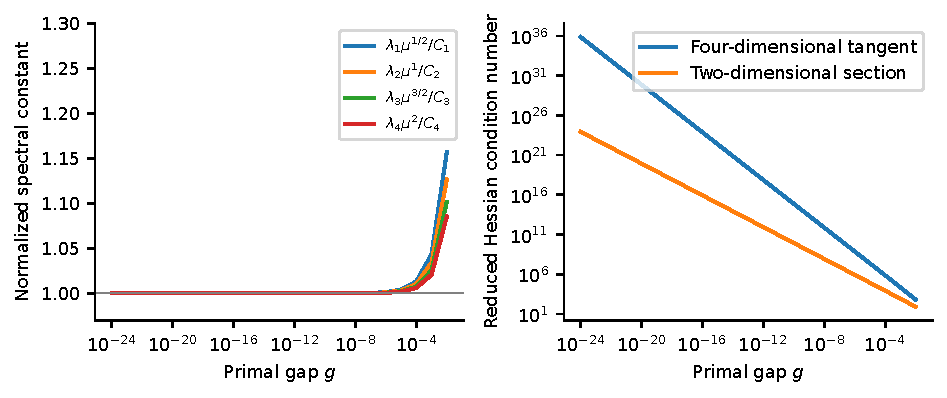
\includegraphics[width=\textwidth]{figures/fractional-sdp.pdf}
\caption{The fractional SDP and its section. Left: the scaled ordered
eigenvalues divided by $C=(\sqrt2,1,\sqrt2,4/7)$, with powers
$(1/2,1,3/2,2)$ of $\mu$. Right: the condition numbers on the two
tangent spaces. Both optimality systems have singularity degree two.}
\label{fig:fractional}
\end{figure}

For the simplex of \cref{prop:simplex-plateau}, the exact log-barrier
center satisfies $x_i=\mu/(c_i+z)$, where $z>0$ is the unique root of
$\sum_i\mu/(c_i+z)=1$. We solve this scalar monotone equation with
70 decimal digits and evaluate the Hessian through its factor.
\Cref{fig:lp-numerics} shows the inverse-square regime giving way to the large limiting
plateau when $g$ falls below $\vartheta$.
For the compact degenerate LP of \cref{ex:degenerate-lp}, direct centering
gives, at $\mu=10^{-9}$,
$\mu^2\lambda_{\min}\approx0.24888160$ and
$\mu^2\lambda_{\max}\approx1.14289068$, consistent with the proved
limit and $\kappa(L)\approx4.59210571$. The full sequence and its
centrality residuals are supplied in the data package.

\begin{figure}[tb]
\centering
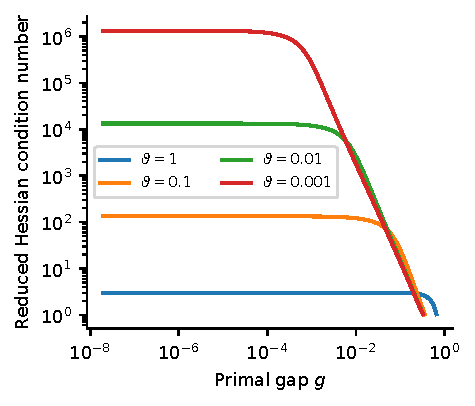
\includegraphics[width=.49\textwidth]{figures/simplex-plateau.pdf}\hfill
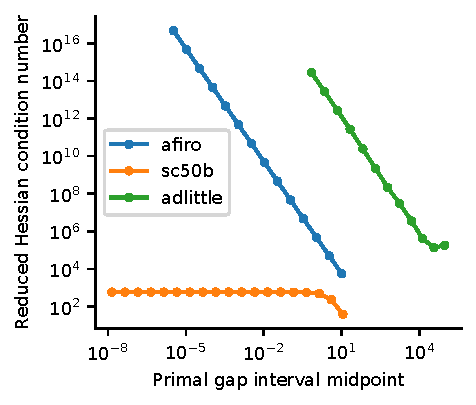
\includegraphics[width=.49\textwidth]{figures/netlib.pdf}
\caption{Left: near-degenerate simplex plateaus for fixed values of
$\vartheta$. Right: accepted finite-gap points for the frozen Netlib
representations. The latter curves are numerical observations; no
asymptotic exponent is fitted to them.}
\label{fig:lp-numerics}
\end{figure}

\Cref{tab:oscillatory} evaluates the exact subsequence in
\cref{prop:oscillatory-barrier}. It records the norm of the discarded
forcing component divided by $g$, and the relative Euclidean error
of the solution obtained by retaining only the strong eigenmode.
The forcing component tends to zero at the proved rate while the
solution error tends to one. This is a direct check of the distinct
residual and solution contracts, not an iterative-solver artifact.

\begin{table}[tb]
\centering
\begin{tabular}{rrrr}
\toprule
$k$ & $g_k$ & $\|\Pi c\|/(g_k\|c\|)$ & Relative solution error\\
\midrule
1 & 1.87e-03 & 0.01000003 & 0.93680040 \\
2 & 3.49e-06 & 0.01000000 & 0.99999976 \\
3 & 6.51e-09 & 0.01000000 & 1.00000000 \\
4 & 1.22e-11 & 0.01000000 & 1.00000000 \\
\bottomrule
\end{tabular}

\caption{Oscillatory barrier with $\epsilon=0.01$ and
$g_k=\exp(-2\pi k)$. The relative solution error is
$\|H^{-1}\Pi c\|/\|H^{-1}c\|$. Rounded values of one do not assert
exact equality at finite gap.}
\label{tab:oscillatory}
\end{table}

\subsection{Certified benchmark representations and precision screens}

We use three small Netlib LPs \citep{netlib}: \texttt{afiro},
\texttt{sc50b}, and \texttt{adlittle}. The frozen arrays are the result
of HiGHS 1.15.1 default presolve followed by conversion of inequalities
and finite bounds to equality constraints and nonnegative variables.
Their dimensions, from original MPS to presolved model to standard form,
are respectively
$(27,32)\to(7,10)\to(9,18)$,
$(50,48)\to(15,15)\to(15,29)$, and
$(56,97)\to(53,95)\to(55,136)$.
The Hessian uses the Euclidean metric in these final coordinates.
It is not the Hessian of the original MPS representation. The frozen
arrays define the tested instances, so a later presolver version is
not needed for reproduction.

The hypotheses are checked without feasibility tolerances. Every
stored float64 input is interpreted as its exact binary rational.
The package verifies a rational point $x>0$ with $Ax=b$ and a rational
vector $y$ with
\[
 A^\top y+\eta c>0,\qquad \eta\geq0.
\]
For $x\geq0$ in a fixed upper objective sublevel,
$x^\top(A^\top y+\eta c)=b^\top y+\eta c^\top x$ bounds every
coordinate. The certificates use $\eta=0$ for \texttt{afiro} and
\texttt{sc50b}, proving compactness of their feasible sets, and
$\eta=1$ for \texttt{adlittle}, proving compactness of its objective
sublevels. Thus the localized theorem applies to the last instance.
Rational primal and dual feasible points also certify brackets on the
optimal value, with widths approximately $8.2\cdot10^{-12}$,
$9.4\cdot10^{-12}$, and $4.5\cdot10^{-7}$, respectively.

Centering uses an orthonormal nullspace basis $W$ and the Hessian factor
$B=\Diag(x^{-1})W$. Singular values of $B$ give the Hessian eigenvalues
by squaring; Newton solves and decrements use the same factorization.
Each stored iterate is repaired to an exactly feasible rational point
using a fixed nonsingular column basis. We evaluate its objective
exactly and subtract the certified optimal-value bracket. A point is
accepted for the plot only when this gap interval is positive and
has relative width at most $1\%$, the repaired point is positive,
the maximum relative coordinate repair is at most $10^{-4}$, the
scaled equality residual is at most $10^{-12}$, and the \emph{unscaled}
centrality decrement is at most $10^{-5}$. We additionally require
\[
 \epsilon_{\rm mach}\max(n,d)\,\kappa_2(B)\leq10^{-6}.
\]
This last screen is a numerical resolution indicator for the factor
SVD, not a rigorous interval certificate for its singular values.
The exact rational certificates establish the instance hypotheses;
the plotted spectral values remain finite-precision computations.

\begin{table}[tb]
\centering
\begin{tabular}{lrrrrr}
\toprule
Instance & $(m,n)$ & Accepted/attempted & Last gap & $\kappa$ & $\rho$\\
\midrule
afiro & $(9,18)$ & 14/27 & 3.34e-06 & 4.65e+16 & 2.2e-07 \\
sc50b & $(15,29)$ & 19/27 & 1.40e-08 & 5.82e+02 & 6.1e-07 \\
adlittle & $(55,136)$ & 12/27 & 6.80e-01 & 2.81e+14 & 2.5e-09 \\
\bottomrule
\end{tabular}

\caption{Accepted Netlib points and the last accepted point in each
continuation sequence. All 27 attempted points per instance, including
centrality, gap, repair, or spectral-resolution rejections, are retained
in the raw data.}
\label{tab:netlib}
\end{table}

\Cref{tab:netlib} makes the different resolved accuracy ranges explicit.
In particular, the stringent spectral screen stops \texttt{adlittle}
well before its deepest attempted gap. We draw no conclusion about
its limiting condition number from that truncation. The near-degenerate
simplex already proves why a finite observed slope or plateau should
not by itself be treated as an asymptotic classification.

\subsection{Clustered CG and the meaning of stopping accuracy}

To exercise two intervals with many distinct eigenvalues, we generate a
$60\times60$ symmetric matrix from a fixed-seed orthogonal rotation of
30 equally spaced values in $[1,2]$ and 30 in $[g^{-2},3g^{-2}]$.
This is a synthetic spectral test, not a claimed Newton Hessian.
The actual float64 matrix is explicitly symmetrized. CG uses ordinary
float64 matrix-vector products and stops when its recursively updated
relative residual first reaches $10^{-8}$. At that iterate, an 80-digit
solve of the exact real system defined by the stored float64 matrix
and right-hand side supplies the reference solution, relative energy
error, and independently evaluated true residual.

\begin{table}[tb]
\centering
\begin{tabular}{rrrrr}
\toprule
$g$ & Iterations & Recursive residual & True residual & Relative energy error\\
\midrule
1e-01 & 43 & 8.82e-09 & 8.82e-09 & 3.54e-09 \\
1e-02 & 71 & 2.56e-09 & 2.56e-09 & 4.21e-09 \\
1e-03 & 96 & 4.37e-09 & 4.39e-09 & 4.24e-09 \\
1e-04 & 124 & 2.95e-09 & 2.52e-08 & 8.55e-09 \\
\bottomrule
\end{tabular}

\caption{Float64 CG on the synthetic two-interval matrices. The final
two columns use an 80-digit reference calculation for the actual rounded
matrix and right-hand side. The last recursive stopping test does not
certify a true relative residual below $10^{-8}$.}
\label{tab:cg}
\end{table}

The prescribed internal interval ratios are two and three while the
interval separation grows; these ratios precede floating-point matrix
construction and are not exact spectral assertions for the rounded
matrix. \Cref{tab:cg} illustrates the benefit of this structure
and the distinction between stopping metrics. It is not an empirical
proof of the exact-arithmetic degree bound. Indeed, exact-arithmetic
CG terminates in at most 60 steps for these matrices, whereas floating
arithmetic can take more steps because conjugacy is lost. Recomputed
residuals and energy error therefore remain separate reported quantities,
as required by the solver contract in \cref{sec:clustered-solves}.

\section{Discussion}
\label{sec:discussion}

The central-path Hessian is constrained by an object that does not
refer to the barrier: the difference body of the current objective
sublevel. This explains both the matching condition-number law and
the comparison of complete spectra at equal accuracy. Within a fixed
representation and metric, a finite-parameter barrier change cannot
remove a conditioning exponent imposed by sublevel geometry. Uniform
bounds on barrier parameters are essential if the barrier itself varies
with the requested gap.

The resulting geometric distinction is finer than several customary
classifications. A unique optimum does not by itself imply bounded
conditioning outside the polyhedral setting. Conversely, primal
vertex degeneracy does not prevent a positive-definite scaled
log-Hessian limit in an LP. In SDP, an attained fractional error bound
can determine the conditioning exponent, but singularity degree alone
cannot: the paired degree-two systems have different diameter rates.
Full-spectrum width bounds explain why an extreme-eigenvalue ratio
also need not describe the interior spectral scales.

For linear solves, the direction of the forcing and the accuracy
contract remain decisive. On an LP central tail, the weak eigenspace
approaches the optimal-face tangent and the exact Newton forcing has
a small projection onto it. The sharp barrier example shows why this
fact is insufficient for accurate direction recovery after discarding
weak modes. Clustered CG can nevertheless exploit separated spectral
intervals in exact arithmetic. Its conclusion is an energy-error
bound, and the numerical examples expose the need to distinguish it
from a recursively computed residual. Quantum applications require
additional access and output assumptions before either fact can be
converted into a runtime statement.

These are statements about a specified primal operator. They coexist
with useful changes of representation, gap-dependent preconditioners,
and primal--dual formulations whose spectra can behave differently.
The precise comparison established here supplies a common geometric
reference for assessing such changes: it identifies what is forced
by objective sublevels before accounting for the cost and effect of
the linear algebra used to solve the Newton equations.

\bibliographystyle{plainnat}
\bibliography{bibliography}
\end{document}
